\documentclass[12pt, oneside, openany]{book}

\usepackage[T1]{fontenc}
\usepackage{hyperref}


\usepackage{subfig,multicol}
\usepackage[export]{adjustbox}



\usepackage[margin=1in]{geometry}% Change the margins here if you wish.
\setlength{\parindent}{0pt} % This is the set the indent length for new paragraphs, change if you want.
\setlength{\parskip}{5pt} % This sets the distance between paragraphs, which will be used anytime you have a blank line in your LaTeX code.

% Load the basics
\usepackage[english]{babel}
\usepackage[utf8]{inputenc}
\usepackage[T1]{fontenc}
\usepackage{titling}
\usepackage{csquotes}% Recommended
\usepackage{graphicx}

% Page numbers
\usepackage{lastpage}
\usepackage{fancyhdr}
\pagestyle{fancy} 
\lhead{}
%\cfoot{\thepage\ of \pageref{LastPage}}

\usepackage[style=authoryear, backend=biber]{biblatex}
\addbibresource{bibliography.bib} %


\usepackage{amssymb}
\renewcommand{\labelitemi}{$\blacksquare$}


\title{
The role of spatial planning 
\\ in facilitating the implementation of 
\\ Circular Economy practices
\\  in City-Regionss
\\
  \large Applications to Industrial Symbiosis \& 
  \\
  Solid Waste Management
\\  
  \small 25\% Seminar}



% Meta of the document

\author{Phd student: Jonathan E. Cohen
\\ Main supervisor: Lars Marcus
\\ Assistant supervisor: Jorge Gil
\\ Examiner: Meta Berghauser Pont}
\date{June 2020}

\setlength{\droptitle}{-5em}   % This is your set screw

\begin{document}
\maketitle\vspace{-5ex}
\tableofcontents

%\cite{OECD2020}\par
%\parencite{OECD2020}\par
%\textcite{OECD2020}\par

%%%%%%%%%%%%%%%%%%%%%%%%%%%%%%%%%%%%%%%%
\chapter{Global sustainability, Cities and Circular Economy}
%%%%%%%%%%%%%%%%%%%%%%%%%%%%%%%%%%%%%%%%
Environmental pressure and threats are challenging governments all over the world. The Sustainable Development Goals and Paris Agreement are important landmarks in human history that recognize that joint effort is needed to achieve not only environmental but also economical and social goals.\par
As the world is becoming more urban and the majority of people are expected to be living in cities, the role of urban and regional planning is becoming crucial to achieve a sustainable future. Local governments, institutions and other stakeholders are engaging in finding novel ways of maximizing the benefits of urbanization while reducing the negative impacts.\par
Circular Economy practices and ideas have been gaining momentum and are perceived a viable solution to mitigate environmental deterioration. In academia, the concept is being scrutinized and the real implications of adopting these practices are being explored.\par
In this context, growing effort is being allocated to translate Circular Economy strategies to cities. In the past years, there is evidence that local authorities are exploring how to incorporate Circular practices into urban planning. 

\begin{figure}[h!]
    \centering
    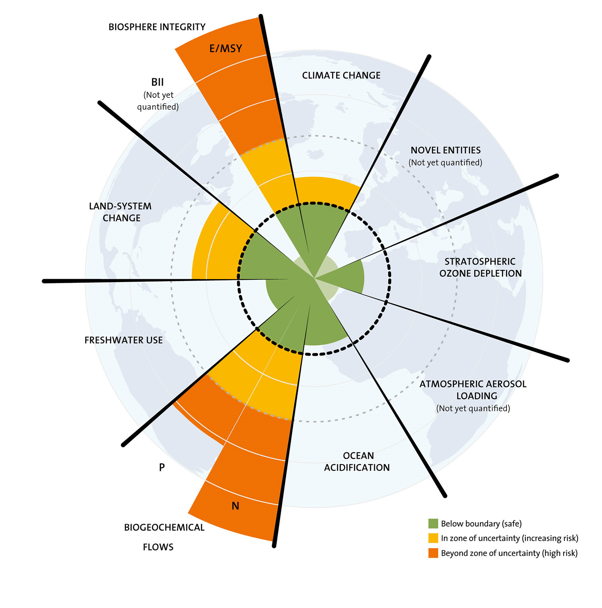
\includegraphics[width=0.5\textwidth]{sections/asset/boundy.PNG}
    \caption{Planetary boundaries. Consuming beyond Earth's bio-capacity of regeneration}
    \label{fig:badbad}
\end{figure}



%%%%%%%%%%%%%%%%%%%%%%%%%%%%%%%%%%%%%%%%
\section{Call for action}
%%%%%%%%%%%%%%%%%%%%%%%%%%%%%%%%%%%%%%%%
Extraction of natural resources surpasses the Earth's bio-capacity of regeneration and in order to maintain current consumption patters, 1.8 Earths are needed. Although, it's controversy  \parencite{Blomqvist2013, Eading1999, Rees2013, Giampietro2014} the Ecological Footprint (EF) calculation is a simple concept that gain media acceptance. International recognized organizations such as United Nations (UN) or World Wildlife Found continue to utilize the metric to indicate an illustrative estimation of the date when humans enter in a environmental deficit because the Earth's will no longer be able to regenerate. This is known as the Earth Overshot Day and from 2005 until 2018 this days were reached by the month of august. In 2018, the Earth Overshot Day was the 29th of July. \par

In 2009, the Stockholm Resilience Centre developed the Planetary Boundaries (PB) framework to define the limits within humanity can safety operate. The research identified nine systems and safety operating boundaries, where the Earth System (ES) will remain stable and consequently life on earth wont be at risk. Thanks to the scientific efforts of this research group, in 2015 it was estimated that life of Earth was already operating beyond four of those limits. \parencite{Steffen2015}.\par

Mobilized to revert the current scenario and move forward in building a global sustainable future, in 2015 world leaders agreed adopt the 2030 Agenda for Sustainable Development and the Sustainable Development Goals (SDGs). In contrast with the  Millennium Development Goals (MDGs), which mainly represents a fight against poverty, the commitment for the SDGs demands actions to be taken from all nations across the globe. A year later, the Paris Agreement was signed with the long term objective to keep global temperatures above 1.5 pre-industrial levels. This would only be achieved by cutting off emissions drastically and more efficient use of resources. \par

The Sustainable Development Goals represent an unprecedented milestone in the history of humankind. For the first time, leaders agreed to allocate resources and efforts towards 17 Goals and 169 targets. In order to move forward in global and national sustainability all countries need to make progress in all 17 Goals. Given the complexity of these systems, synergies and tensions have been identified among the SDGs and in order to make the most out of the policies, investments and efforts, resources need to be mobilized as efficiently as possible. \par

The agreement at the UN General Assembly in 2015 constituted a historical landmark in humanity. For the first time in history diverse world leaders agreed upon a general set of goals to work towards and signed the Agenda 2030 for Sustainable Development (Agenda 2030). In contrast to the Millennium Development Goals (MDGs), in this opportunity the Sustainable Development Goals (SDGs) represented a commitment that involves all countries, no matter the level of development, wealth or industrialization.  Currently 17 Goals are associated with 169 targets and a total of 232 indicators. In December of the same year, in the UN Framework Convention on Climate Change (UNFCC) the Paris Agreement (COP21) was signed to mitigate greenhouse gases (GHGs) emissions and avoid average temperature increases of 1.5C above pre-industrial levels. Both agreements show evidence of national governments and global leaders acknowledging that current practices are unsustainable and if no actions are taken to revert current trend, our support system, might become unstable and threat life on earth.\par


%%%%%%%%%%%%%%%%%%%%%%%%%%%%%%%%%%%%%%%%
\section{Cities and regions to attain the SDGs}
%%%%%%%%%%%%%%%%%%%%%%%%%%%%%%%%%%%%%%%%

Although the surface covered by cities is only cover 2\% of the earth, these areas host almost half of the global population and are responsible for 80\% of the global C02 emission, consequently; "The battle for sustainable development will be won or lost in cities" \footnote{https://www.un.org/press/en/2017/dsgsm1080.doc.htm} \footnote{https://www.undp.org/content/undp/en/home/blog/2018/battle-for-sustainable-development-will-be-won-in-cities.html} \footnote{https://www.weforum.org/agenda/2015/09/the-fight-for-sustainable-development-will-be-won-or-lost-in-our-cities/}.  \par
In 2016, the first post-Agenda2030 summit that took place was the UN Conference on Housing and Sustainable Urban Development, UN Habitat III (UNHIII), where the main objective of the Conference was to debate the details of the SDG \#11 (Make cities and human settlements inclusive, safe, resilient, and sustainable). The New Urban Agenda was the main output of UNHIII and it represents a step forward in localizing the SDGS and serves as a guide to local and regional authorities to promote sustainable practices.  \par
According to the OECD, in order to achieve at least 105 of the 169 targets local and regional engagement is required \parencite{EuropeanCommission2018, OECD2020}. Moreover, it is stressed that territorial indicators and high quality granular data are essential to move forward in the process of localizing the SDGs. Since nowadays in most countries, local governments are accountable for its citizens well-being, localizing the SDGs imply much more than implementing the SDGs, but will require active participation of local governments in defining the policies needed to achieve the SDGs targets. \par
In the light of the year 2020 events, it has become clear that much urban and regional research is needed to understand city dynamics, how they interact with other urban settlements and resource hubs. Definitely, cities (and the network of them) will play a crucial role in achieving the SDGs and planning tools are needed to ensure enhance resiliency against diverse threats.   



\section{On the importance of Circular Economy}
According  the Circularity Report gap \parencite{CircleEconomy2020}, "Today, the global economy is only 8.6\% circular — just two years ago it was 9.1\%. There are reasons for this negative trend, but the result remains the same: the news is not just bad, it is worse. This negative trend can be explained by three key related, underlying trends: high rates of extraction; ongoing stock build- up; and, increasing (but still low) levels of end-of- use processing and cycling. These underlying trends are deeply embedded within the ‘take-make-waste’ tradition of the linear economy — the problems are hardwired. As such, the outlook for closing the circularity gap looks bleak under the dead hand of business as usual. We desperately need transformative and correctional solutions; change is a must."\par
Implementing CE strategies can be used to successfully meet several of the SDGs. Direct positive effects are associated with SDGs 7, 8, 12, 6 and 15 \parencite{Schroeder2018}. 

\begin{figure}[h!]
    \centering
    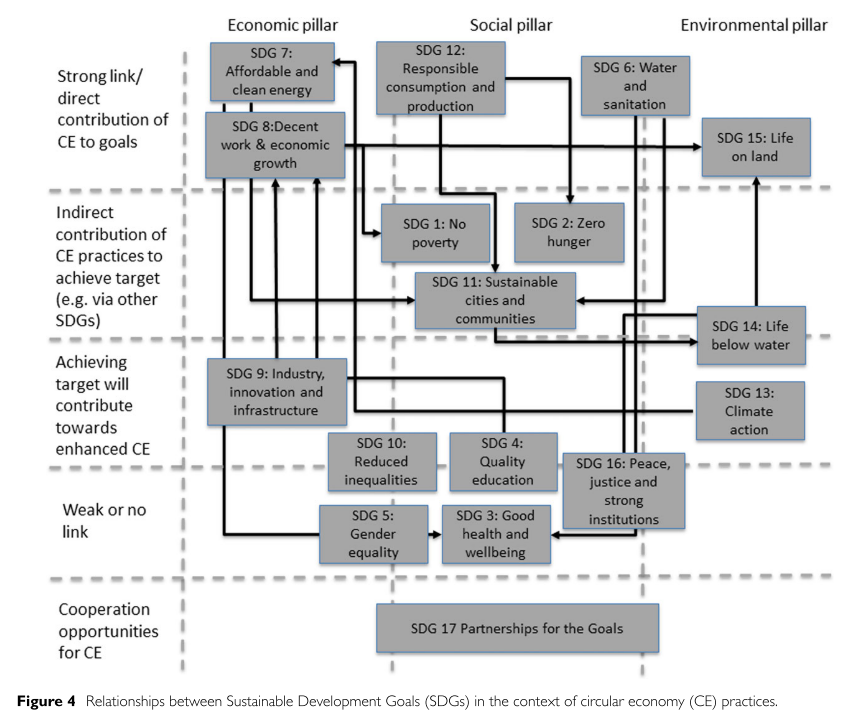
\includegraphics[width=0.7\textwidth]{sections/asset/ce_relation.PNG}
    \caption{Circular economy contributions to SDG}
    \label{fig:badbad}
\end{figure}


According to a study conducted by the Ellen MacArthur Foundation and McKinsey in 2015, adopting a circular economy approach could boost the continent’s resource productivity by 3\% by 2030, generate cost savings of 600 billion Euros a year and bring 1.2 trillion Euros in other non-resource and externality benefits. The key areas of benefit are mobility, food and buildings. Another 2015 study by the United Kingdom’s Waste and Resources Action Programme found that a circular economy has the potential to create 1.2 to 3 million jobs in Europe by 2030. \par


Ellen McArthur Foundation defines CE as a \cite{systemic approach to economic development designed to benefit businesses, society, and the environment. In contrast to the ‘take-make-waste’ linear model, a circular economy is regenerative by design and aims to gradually decouple growth from the consumption of finite resources. After defining what an economy actually is, this learning path explores the nuances of the concept of a circular economy, including the difference between biological and technical materials, the different opportunities that exist to keep materials and products in use, and the history of the idea.} \par
Still, under the view of certain academics the concept is still evolving and since is still in early stages of development, much research is needed to explore its meaning, applications and implications \parencite{Ghisellini2016}. According to \textcite{Kirchherr2017} the main aim of the CE is considered to be economic prosperity, followed by environmental quality; social equity and future generations is barely mentioned. \par

\begin{figure}[h!]
    \centering
    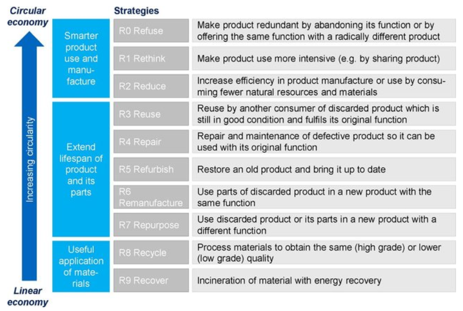
\includegraphics[width=0.7\textwidth]{sections/asset/rs.png}
    \caption{Circular economy vs linear economy strategies}
    \label{fig:badbad}
\end{figure}


The concept of CE has been introduced to cities and some authors have trying to translate what does this means for urban and regional planning \parencite{Williams2019}. 

\begin{figure}[h!]
    \centering
    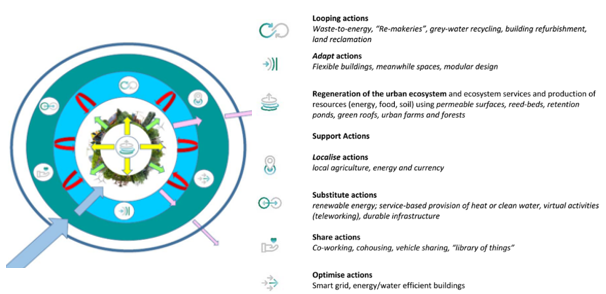
\includegraphics[width=0.7\textwidth]{sections/asset/city.PNG}
    \caption{Circular economy conceptualization for cities}
    \label{fig:badbad}
\end{figure}

%%%%%%%%%%%%%%%%%%%%%%%%%%%%%%%%%%%%%%%%%%%%%%%%%%%%%%
\chapter{Theoretical background}
%%%%%%%%%%%%%%%%%%%%%%%%%%%%%%%%%%%%%%%%%%%%%%%%%%%%%%

In this section I will organize and discuss the main theoretical building blocks that will be required to overcome the challenges previously identified and bring answers to the inquires this dissertation have raised. \par

\begin{figure}[h!]
    \centering
    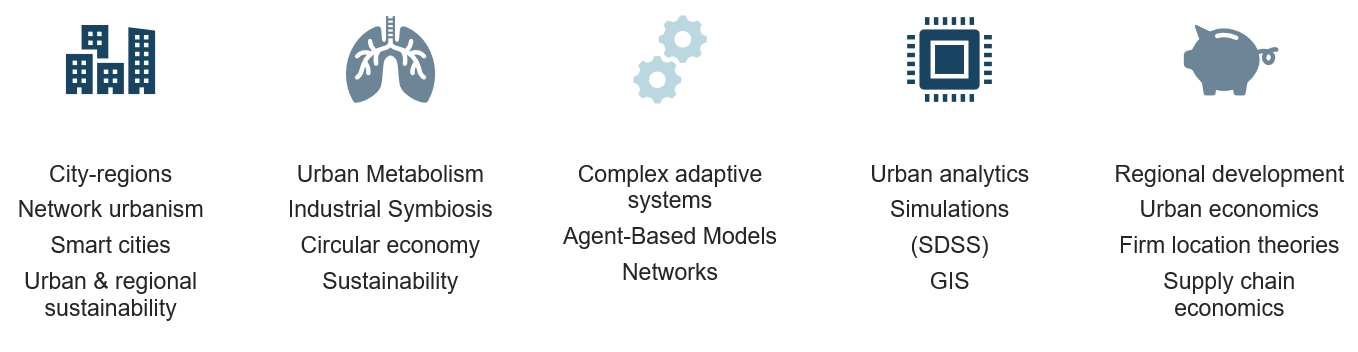
\includegraphics[width=0.8\textwidth]{sections/asset/theo.PNG}
    \caption{Theoretical background. Main research domains}
    \label{fig:theo}
\end{figure}

In order to make a substantial contribution as an interdisciplinary research and avoid falling in superficial -or wrong – analysis it would be crucial to become aware and build knowledge in different domains. Consequently, it is important to have a clear conceptual idea of the different definitions, assumptions, perspectives and biases carried within each of the fields to work with.
This dissertation will be contributing to fill gaps and build knowledge bridges between the following 3 disciplines:\par

\begin{enumerate}
    \item The goals and strategies: Sustainable development(SD)
    \item Theoretical and conceptual framework: Urban and regional science (URS)
    \item Application to real world problems: Urban \& regional planning
\end{enumerate}

In the intersection of some these big fields of research it is already possible to find advancements. However, as the outcomes of this research become clearer, also the tensions between the fields I will be trying to bridge will arise to the surface. It will become evident that the results are not contributing equally in all these fields. \par

Although, this research is borrowing from these fields simultaneously, in first place \textbf{Sustainable Development (SD)} and the contribution of \textbf{Circular Economy (CE)} as a potential strategy will be explored. Under the umbrella of circular economy, the field of industrial ecology and urban metabolism can offer theoretical frameworks to study the problems of resource efficiency. This exploration, naturally leads to 2 mainstream practices (i) \textbf{Industrial Symbiosis (IS)} and (ii) \textbf{Solid Waste Management (SWM)}. \par  

In second place, these two of how to handle resources or waste flows, partially overlaps with a well established branch of urban and regional economics. In economics and more specifically, \textbf{New Economic Geography (NEG)} has a long tradition of dealing with the location of industries, logistics and supply chains transport economics.\par

The third knowledge stream is rooted in \textbf{urban planning}. As so, in contrast with the previous ones, it starts to detach from theory and brings a specific tool-set of analytical methods to materialize the concepts highlighted before. This last domain fills the research with the necessary tools to articulate the dialogue between the first and second main areas of knowledge. \par 
This PhD will be borrowing concepts, frameworks and theory from (1) \& (2), and the outcomes will contribute to build tools and expand the knowledge of how to plan sustainable city-regions. \par















% \section{On the importance of Circular Economy}
% What is Circular Economy? Give a definition 



% Implementation worldwide still in early stages [1] 
% Metrics and other assessment methods will play a key role in understanding [2] 
% Main aim of the CE is considered to be economic prosperity, followed by environmental quality; social equity and future generations is barely mentioned [3] 
% 7 strategies are conceptualized to implement CE in cities [4]

% [1] (Ghisellini et al, 2016)
% [2] (Blomsma & Brennan, 2017)
% [3] (Kirchherr, 2017)
% [4] (Williams, 2019)





% Urban planning contributes to simulate circular processes at different scales through a systemic approach and evoking the approaches of industrial ecology [1]
% Urban metabolism as a planning tool to identify opportunities for CE initiatives and monitoring of progress [2]
% Understanding of the spatial relationships between a city and its hinterlands and global resource networks is critical for urban policy makers [3]


% [1] (Girard et al., 2019) 
% [2] (Kalmykova & Rosado, 2015)
% [3] (Kennedy et al., 2007) 





% \begin{figure}[h!]
%     \centering
%     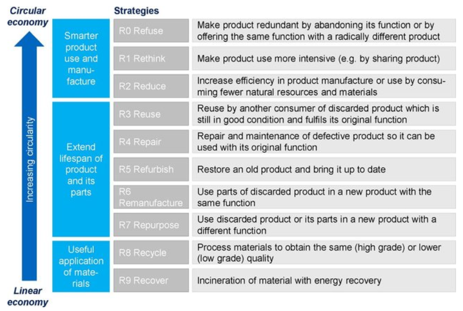
\includegraphics[width=0.7\textwidth]{sections/asset/rs.png}
%     \caption{Circular economy ladder of strategies}
%     \label{fig:badbad}
% \end{figure}





\chapter{Problem definition: Waste material in city-regions}

Environmental degradation, miss usage of resources, and pollution are not virtual or intangible processes, they are tied to specific locations. There is a reason behind the geographical structure of these events which also deserves to be explored. By introducing the spatial dimension to the analysis, planning for better city-regions becomes spatial planning. \par

The problem of improving the quality of human settlements is complex and requires of a holistic approach to make effective contributions (Figure \ref{fig:complex_sdg}). There is a significant amount of interactions between the goals and in order to plan for a more sustainable places, these relationships need to be explored \parencite{Eurostat2019, Miola2019,euc2019}. By systematically looking at how these goals relate to each other, synergies can be enhanced, and tensions taken into consideration. Planning as a general practice will deal with evaluating and organizing what is the best course of action to meet a target. \par
%
Monitoring KPIs is an important activity, they provide information about the result of a process (or processes). By them self, they do not contain information about how a system works or is performing, but information about the working of a system are important for Planning purposes. \par
%


\begin{figure}[hbt!]
    \centering
    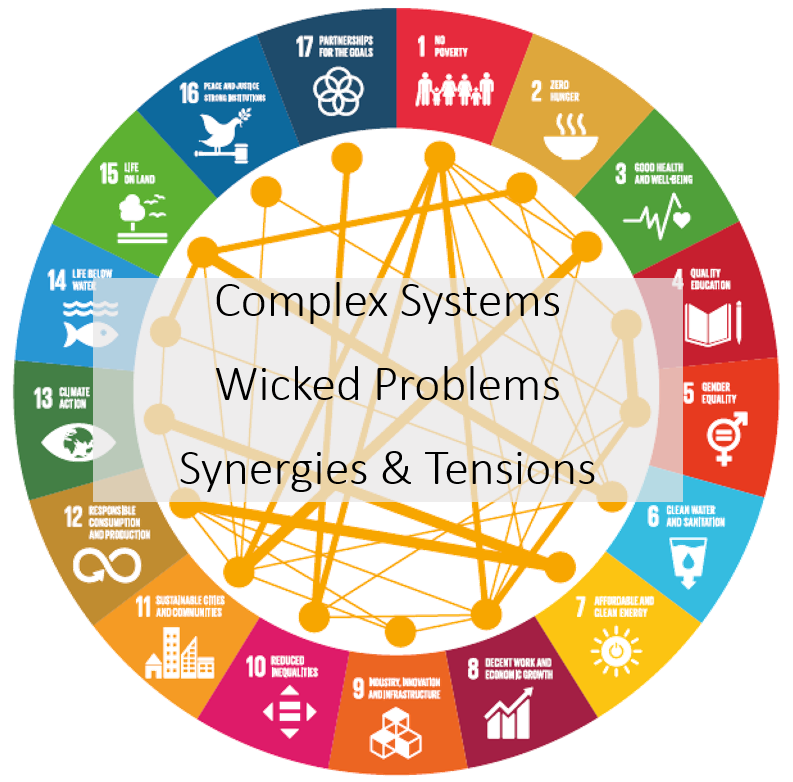
\includegraphics[width=0.45\textwidth]{sections/asset/3_complex.PNG}
    \caption{SDGs: Complex and Wicked Planning problems \parencite[pp. 30]{Eurostat2019}}
    \label{fig:complex_sdg}
\end{figure}
%

For the purpose of this exposition, the idea that a city-region works as a factory will be used to illustrate the general problem being faced here. Now, let's imagine that the owner of a factory wants to increase the production, she would start to ask questions about how much is being currently produced and then start to monitor the amount of inputs requested. By solely looking at these variables, much planning cannot be done. Decisions about the amount and the combination inputs could help to enhance production, but soon more question about the processes behind production will arise. More information about the components of the factory will be requested, number of employees, salaries, energy consumption, machines used, and so forth. As more and more detailed KPIs about the production are being monitored, the processes of production will be revealed. \par

A city is not a factory. Besides many other differences, in a factory the processes are linear. Inputs are transformed step by step in a linear process. Each step is related to the previous one and so forth. Once a part moves forward in the production line, it never goes back and affects previous process. Social and economic systems are complex and any performance indicator needs to take into account the complexity of these systems. 
In order to meet the targets, it has never been clearer that spatial planning is necessary. In some urban domains such as transport, there has been long tradition of exploring the relation between land use, mobility and socio-economic activities. As a result of data availability and it's natural proximity to geography, transport systems have been spatially planned for long time. New data sources and technological innovation can contribute to enhance the study of space in other urban domains. \par

\textcite{Rittel1973} argue that in \textit{`large and interconnected network systems(...), it has become less apparent where problem centers lie, and less apparent where and how we should intervene even if we do happen to know what aims we seek'}. Only after unpacking the systems interrelations, it would be possible to meet targets that are sustainable over time and minimize undesirable side effects.\par

Because most of these are urban or regional processes occurring in specific locations, spatial planning becomes the tool to help to define the specific set of actions in the space to affect performance.  \par

To sum up, to modify the performance of a complex system it is needed to:


\begin{enumerate}
    \item Understand the processes within the system
    \item Understand how that system interacts with other systems
    \item Understand the spatial-temporal properties 
\end{enumerate}


\section{Problem statement}


The following major issues must be considered in discussing the management of solid wastes: \parencite{CDR2005}\par

\begin{enumerate}
    \item increasing waste quantities
    \item wastes not reported in the national MSW totals
    \item lack of clear definitions for solid waste management terms and functions
    \item lack of quality data
    \item need for clear roles and leadership in federal, state, and local government
    \item need for even and predictable enforcement regulations and standards
    \item resolution of inter county, interstate, and inter country waste issues for MSW and its components
\end{enumerate}


Despite the many advantages obtainable from developing an effective recycling process, experience has shown that several barriers hinder the development of effective recycling markets \parencite{CDR2005}:

\begin{enumerate}
    \item Lack of consumer awareness about recycled products
    \item Lack of consumer confidence in the quality of products made from recycled materials
    \item The social costs and benefits are not reflected in the price of products. Despite environmental advantages, recycled products are generally more expensive than their counter- parts made from virgin materials
    \item The high cost of transporting recyclables from the point of collection in many cities and rural areas to centralized processing plants
    \item Uncertainty about supply-and-demand stability of recyclable products deters financial investment in facilities using recycled materials
    \item Recovery and sorting of certain recyclable materials such as plastics, oil, tires, and demolition products is difficult, and technological improvements are necessary to increase the efficiency of recovery.
\end{enumerate}







\section{Challenge}
The importance of the SDGs and its KPIs is recognized as a step forward to meet the global sustainability. Yet, there is a link missing between how things are done in practice (in the territory) and what the SDG indicators are addressing. This gap needs to be bridged. There is a challenge raised by SDG11, to build better human settlements, and this means dealing with space. dealing with the spatial planning of places. In order to plan better city-regions there is a need of spatializing, modelling and understanding how space (the specific location of places and events) can be adequately incorporated into valuable information for planning. \par

As described above, KPIs do not give information about the set of actions needed to create sustainable places or improve how resources can be used more efficiently. Studying and understanding the interaction between the indicators is crucial, but also where  and when in time these events happen is important and not trivial. \par

Moreover, since generally speaking these KPIs are aggregated at national levels (rarely broken down into smaller geographical units), it becomes difficult for local governments to plan for sustainable development. \par 
Finally, the metrics used to evaluate progress in sustainable development are a-spatial and do not take into consideration how different places interact or the the role of places. Since, cities are important for global sustainability, local and regional authorities need to plan better regions and the demand for metrics that can capture what is actually happening in their territories is necessary. 



\begin{figure}[h!]
    \centering
    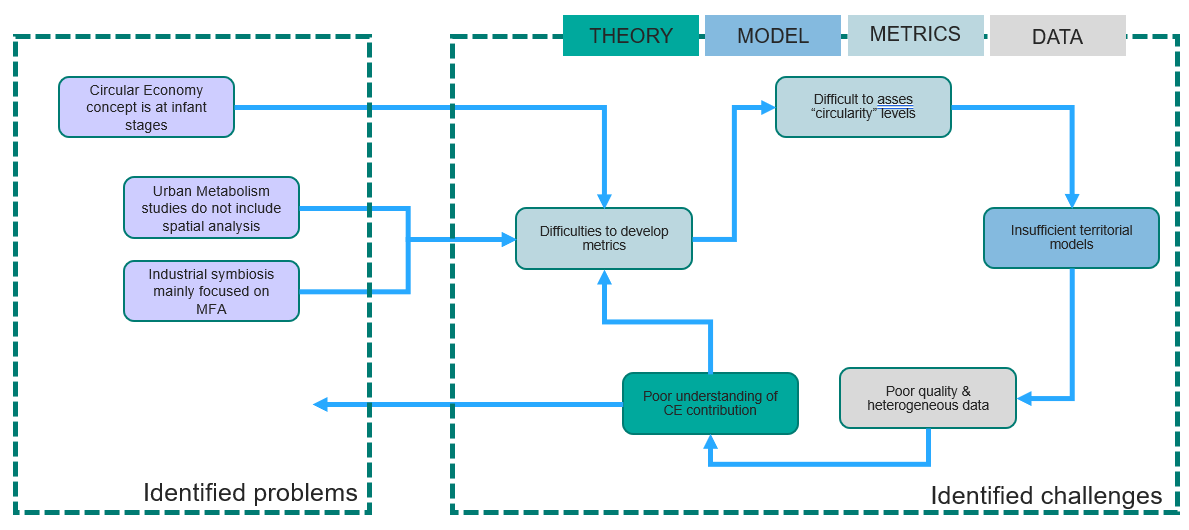
\includegraphics[width=0.8\textwidth]{sections/asset/challenge_probs.PNG}
    \caption{Problem and challenge identification}
    \label{fig:problems}
\end{figure}



\chapter{Research Goal, Aim and Objectives}
Based on the environmental challenge, (minimize the environmental impacts) the state of the art and the identified knowledge gap, the \textbf{goal of this thesis will be to understand the the role regional spatial planning can play in facilitating circular economy practices}. %re-write this. pay attention to facilitating
By describing and analyzing how secondary resources (waste) flow in a city-region it will be possible to explore how the location of different socio-economic activities contribute to closing material loops. \par
By exploring the relevance of the spatial patterns, this project will contribute to understand how planning instruments could be integrated with material flow analysis.\par


\begin{figure}[h!]
    \centering
    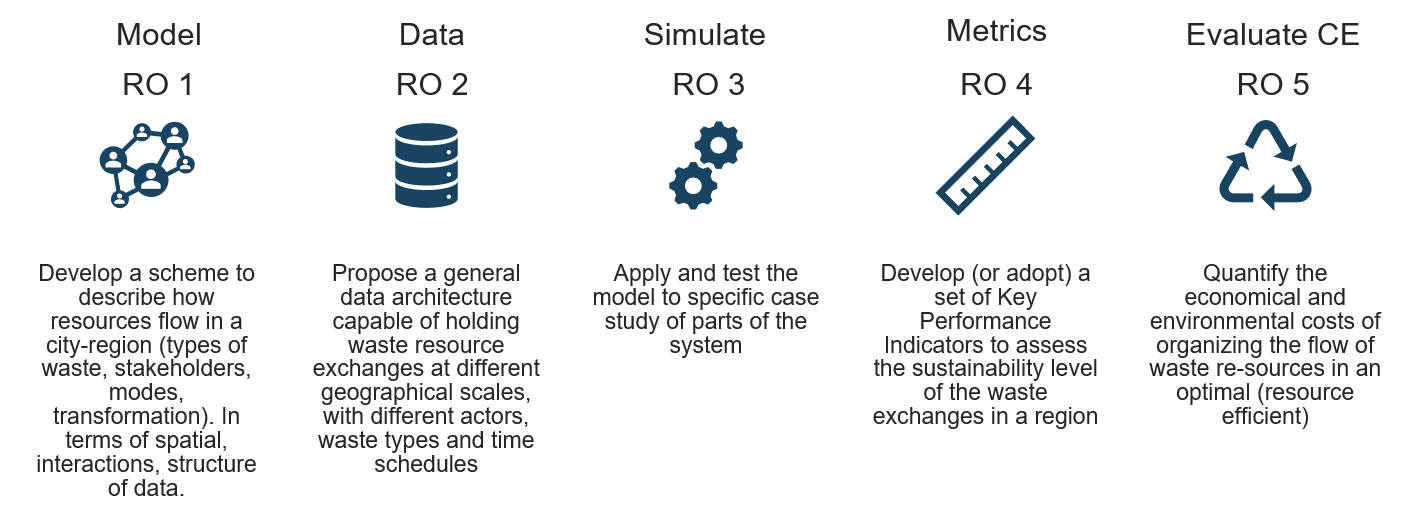
\includegraphics[width=0.8\textwidth]{sections/asset/ros.PNG}
    \caption{Short description of research objectives}
    \label{fig:research objectives}
\end{figure}

Most of the socio-economic process that currently exist, are still part of the so-called linear economy model, where a raw material is produced, then sold and later disposed as waste; a by-product of production or consummation that in most of times does not have any economical value for society. As explained before the paradigm of Circular Economy implies that there are different strategies to be implemented make this process to close the loop of resources between production and consummation. The ecosystem of strategies to be adopted under this new paradigm is vast and need to be applied in the 3 stages of a life of any product: at the stage of development, using local and waste resources, maximizing the life span of a product and ensuring that after the product is no longer used, its components could be easily dismantled and reused again. \par
In this project, the contribution to the Circular Economy paradigm will be focused on trying to close by exploring the role of urban and regional planning. \par
From economic geography theory it has been acknowledged that the location of some economic activities follow certain rationale. Some industries tend to experience different benefits by co-locating one next to the other. Industrial and Eco-industrial parks has shown, that they can be used as tools to increase production efficiency. Water, electricity and other resources are shared or used in a smarter why which result in symbiotic relationships. \par
Since not all socio-economic activities are co-located, but sparse in space, resources and waste resources flow in space creating a demand for transporting these materials. \par
Thanks to the advancements in computing and digital technologies, now more than ever it has become easier to know what and how much is being produced, what and how much waste is being produced and also, we might be at the stage of knowing where these events occur. The possibility of having this information, creates an enormous potential to study the role of space to reduce waste creation. By having the possibility of mapping, analyzing and simulations different scenarios, practitioners and policy makers can be offered analytical tools to work towards more sustainable futures. \par

\section{Research objectives}

In order to  successfully reach the goal of this research, the project the following objectives:
\begin{enumerate}

    \item 
    Develop an information scheme to describe how resources flow in a city-region. The scheme should be able to hold information about different waste types, stakeholders, waste uses, how is transported and other attributes. The scheme developed should hold geographical information and how the different actors and components in the system relate to each other.
    
    \item 
    Propose a general data architecture capable of holding waste resource exchanges at different geographical scales, with different actors, waste types and time schedules. 
    
    \item 
    Apply and test the spatial model  %(datamodel)
    to an specific case study. The case study will contribute to test to what extent the data model is capable of holding information of a part of a system. The case study must be geographically constrained, but also in terms of the waste typology. 
    %--> TASK: Identify, collect, organize data to be used to describe how resources flow in a city-region --> TASK: Quantify, describe, map the waste resources flowing in a city-region. TASK2: Model and simulate how waste resources should flow to attain high levels of sustainability by maximizing the use of waste flows. 
    
    \item 
    Develop (or adopt) a set of Key Performance Indicators to assess the sustainability level of the waste exchanges in a region. These metrics should be able to capture the performance of a region or urban area in terms of usage of waste materials. 
    
    \item Quantify economical and environmental costs of organizing the flow of waste resources under different scenarios. By understanding and comparing how different scenarios perform different, the learning could be used to plan better city-regions.

\end{enumerate}



\chapter{Research Questions}
After acknowledging the main research challenges and defining the knowledge gaps that this research will be working on, in this section the main research question is introduced. Also this main question will be broken down into different sub-questions. This strategy has a twofold advantage, on one hand it helps to define small and achievable tasks and it contributes to fill knowledge gaps of different sorts. As seen before, the knowledge domain of this work stands on the intersection of different and diverse fields and consequently, to move forward in the domain of circular economy and urban planning, research is needed in different fronts. For instance, this research will face problems of how to structure and model information of waste flows and explore what metrics could be used to understand progress in terms of circular economy. By first answering smaller and related questions, by the end of the project a bigger picture with an (or partial) answer will emerge. 

\section{Main research question}
Since cities and the network of them that create regions, are crucial to develop a more sustainable local and global future, the effect of different strategies need to be explored. Since 1970 the concept of circular economy has been gained momentum, firstly among the private sector and in the last 5 to 10 years by policy makers. Nowadays, the debate has been also picked up by academia where the concept is being scrutinized. The ideas of circular economy have cross pollinated across a diversity of domains and the urban domain is no exception. Consequently, this creates a variety of questions in the intersection of many knowledge areas. \par
Taking into consideration the research aim and objectives stated above, this research project will be focused on trying to answer the following general research question: \par 

\textbf{\textit{What is the role of spatial configuration in facilitating re-use of waste materials in a city-region?}} % stick to the spatial configuration - and depart from regional planning and institutional political 
% \textbf{\textit{How can spatial urban analysis be integrated into the domain of waste material flow to support planning practices in developing sustainable city-regions?}} \par



\begin{figure}[h!]
    \centering
    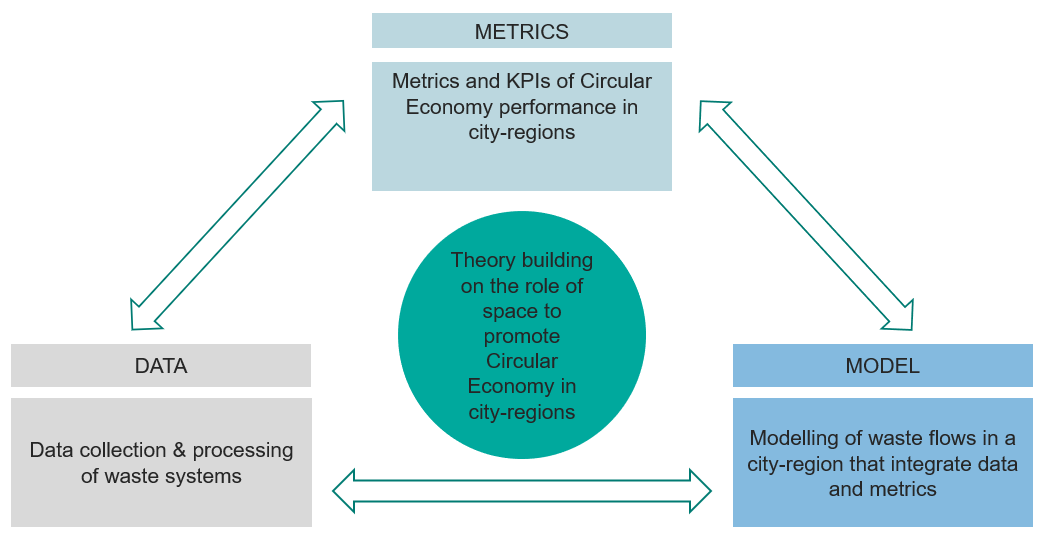
\includegraphics[width=0.8\textwidth]{sections/asset/blocks.PNG}
    \caption{Research components of the project}
    \label{fig:research_bloacks}
\end{figure}



\section{Sub-questions}
In order to bring answers to this main question and contribute to shorten the knowledge gap identified above, the main question is broken down into 9 sub-questions that fall inside 4 different categories of equal importance. As the research project progresses, and specific tasks are accomplished, these sub-questions will be answered. Eventually, after exploring these different sub components an answer to the main question will emerge. \par
Before attempting to answer the main research question,  a set of equally important building blocks are found to be necessary.

\subsubsection{Metrics \& KPIs}
    After reviewing work done in the field of urban metabolism, industrial ecology and or industrial symbiosis, it became clear that most of tools used to analyse the performance of city or region in terms of material use was not incorporating the geographic dimension. The use geographical tools and exploration of how different spatial patterns may (or might not affect) the performance of a system was missing. As a response in order to move forward in the field of circular cities, it is important to answer the following sub questions:\par
    
    \begin{itemize}
        \item \textit{\textbf{RQ1.1: }What KPIs are used to evaluate circular economy in a city-region?}
        \item \textit{\textbf{RQ1.2: }What information is being used to describe and assess circular economy status?}
        \item \textit{\textbf{RQ1.3: }What other metrics can be derived from the spatial configuration of waste flows?}
    \end{itemize}
    
    
\subsubsection{Data models \& simulations}
    Since one big aspect of urban and regional planning is being able to plan for future scenarios or understand how different spatial patterns can influence urban activities, simulations and spatial models are becoming important components of the planning toolkit. For these models to be used by practice they need to be geographic specific. Tools such as Spatial Decision Support Systems (SDSS) and GeoDesign are helping planning agencies to develop better city-regions. Still there is much work to be done in this domain, specifically when it comes to waste materials and how they flow in an a region. On one hand, in these models the location of socioeconomic activities is not taken into consideration, also, in some cases the model used lack the transparency to be used by other researchers or practitioners and lastly, data is still coming from different sources and the field of waste resources has not yet reached a maturity level were there is single data and modelling standard. In transport services, since the development and massive adoption of data standards, there has been a proliferation of different tools and uses for this data. In response to this challenge, the following set of sub-questions will be answered in this project. 
    

    \begin{itemize}
        \item \textit{\textbf{RQ2.1: }How to model the fluxes of waste materials within a city-regions?}
        \item \textit{\textbf{RQ2.2: }Can a general data model hold different types of waste?}
        \item \textit{\textbf{RQ2.3:} How can a spatial model be used to asses the performance in terms of material flow?}
    \end{itemize}


\subsubsection{Data}
    Granular information availability has been growing in the last 5 years. Nowadays, more frequent, more diverse and more precise data is being collected from different sources. Yet, the advancement is not equally distributed across fields. For example, urban transport is one of the most advanced fields were computer science is being applied. The amount of analytical tools and planning applications in transport has shown the importance of collecting and using digital tools to solve urban problems. Yet, when it comes to solid waste, industrial waste or any other sort of by-product, data is being collected at aggregation points. We are capable of knowing how much waste is produced by a country, a region or city  (sometimes) but there are still many data gaps, that does not allow the field to take advantage what digital tools can offer. The lack of data erodes the possibility of creating new tools, and the lack of tools does not create the necessary demand to collect data. 
    
    \begin{itemize}
        \item \textit{\textbf{RQ3.1: }How data of waste flows could be collected to validate the models?}
    \end{itemize}



\subsubsection{Theory}
    Finally, but at the core there are big theoretical questions that could be answered. As the urban digital toolkit continues to expand to waste, by-products or secondary resources, theoretical answers will be able to be answered. As models, data collection and indicators become more precise  and sophisticated, theoretical questions will be answered. By pushing forward the knowledge frontier in the 3 components described above, the possibility of building testable theories in the field of waste materials and urban metabolism will be unlocked.  
    
    \begin{itemize}
        \item \textit{\textbf{RQ4.1: }What are the spatial parameters that contribute to close the loop of resources?}
        \item \textit{\textbf{RQ4.2: }How realistic is to close-loops locally?}
    \end{itemize}



%%%%%%%%%%%%%%%%%%%%%%%%%%%%%%%%%%%%%%%%%%%%%%%%%%%%%%%%%%%%%%%%%%%%%%%%%%%%%%%%%%%%%%%%%%%%%%%%%%%%%%%%%%%%%%%%%%%%%%%%%%%%%%%%%%%%%%%%%%%%%%%%%%%%%%%%%%%%%%%%%%%%%%%%%%%%%%%%%%%%%%%%%%%%%%%%%%%%%%%%%%%%%%%%%%%%%%%%%%%%%%%%%%%%%%%%%%%%%%%%%%%%%%%%%%%%%%%%%%%%%%%%%%%%%%%%%%%%%%%%%%%%%%%%%%%%%%%%%%%%%%%%%%%%%%%%


    % How can the fluxes of waste materials produced in a city-regions be modelled? (as data and model)

    % What are the data requirements to model how resources flow in a city-region?
    
    % Can a general data model be used to hold different types of waste resources?
    
    % What are the spatial parameters that contribute to close the loop of resources?
    
    % Does space needs to be taken into consideration in the KPIs?
    
    % What KPIs can be used to evaluate the degree of circular economy in a city-region?
    
    % How to evaluate the performance of a city-region in terms of closing loops?
    
    % Are these KPIs taking into consideration the spatial parameters of waste flows?
    
    % What other metrics can be derived from the spatial configuration of waste flows?
    
    % What information is being captured in case studies of waste material flow?
    
    %How desegregated is waste resources data published?
    
    % What tools could be used to capture and feed a model of waste fluxes?
    
    % How realistic is to close-loops locally? 
    
    % Can the loop of resources be fully closed %within the city-regions boundaries?
    
    % How is the flow of waste resources in a city-region being assessed and what key performance indicators are calculated in order to evaluate how sustainable waste materials flow in a region?
    
    % How can the exchange of waste materials between industries in a region be spatially modelled? 
    
    % How should waste materials flow in a region in order to achieve an optimal resource usage? 
    
    % How much would it cost to achieve an optimal flow of waste material at a regional level?
    
    % How would a model that captures the flow of waste materials in a region should look like? What are the necessary attributes needed? What can be learnt by reviewing well documented case studies?
    
    % What are the potential uses of such a model? Can this model structure be also used to model the waste at a city level generated by households and managed by a municipality?
    
    % Do conclusions drawn from a-spatial material flow diagrams are still valid if space and the costs of moving residual material are taken into account?  

    % Does waste sorting and collaboration with urban recyclers improve the efficiency of urban solid waste management systems?

    % How to develop a methodology that can quantify and classify waste generated by house holds?

    % How can IoT be incorporated in waste bins to produce an information feed that can be used by to improve the waste management system?
    
    % What is the role of informal waste collectors in the global south? How can their activity be visualised?
    
    % How can information exchanges between generators and pickers could contribute to increase the recycling rates? 
\chapter{Scope}
In this project, the scope of the research is of extreme relevance. Given the fact that the problem identified and the main research question are general, the scope will contribute to stress the focus and delimit those domains that are beyond the current project.\par
This dissertation will take a quantitative approach to study the urban systems and develop digital tools. Approaching the research questions stated above, immediately reduces the scope of this work, specially as it will become clearer below, when these ideas are intersected with the ideas of circular economy.\par



\begin{figure}[h!]
    \centering
    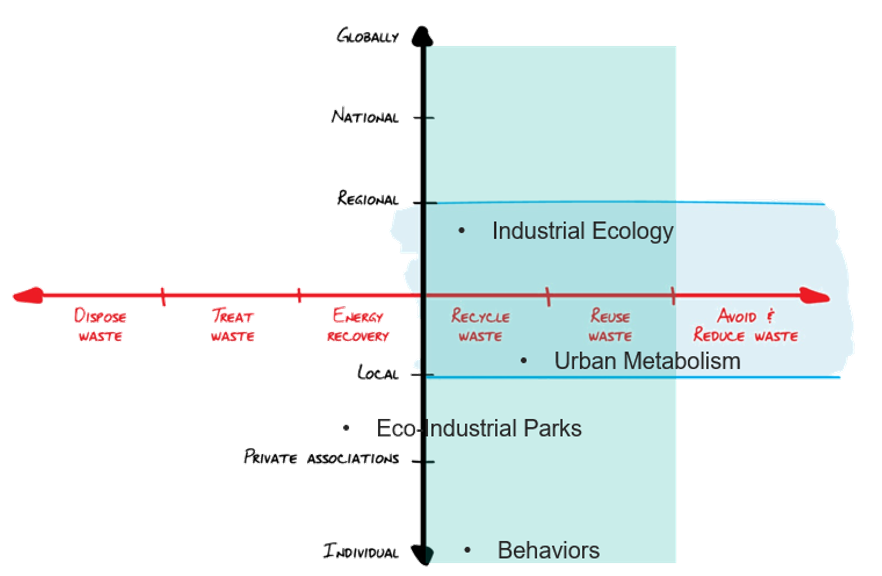
\includegraphics[width=0.8\textwidth]{sections/asset/scopeee.PNG}
    \caption{Scope of the research}
    \label{fig:scope}
\end{figure}



\section{Type of research}
In order to delimit this project and to position this research in terms of the ecosystem of the work done about Circular Economy, the review done by \textcite{Merli2018} is used. In this work different academic articles working with Circular Economy are studied and different categories are suggested. This work is of importance since, it provides a general knowledge of the type of research that is being done and how Circular Economy is approached. In the following table, extracted from this article, different structural dimensions are presented. Each domain contains different analytical categories which are used to study the concept. 

\begin{figure}[h!]
    \centering
    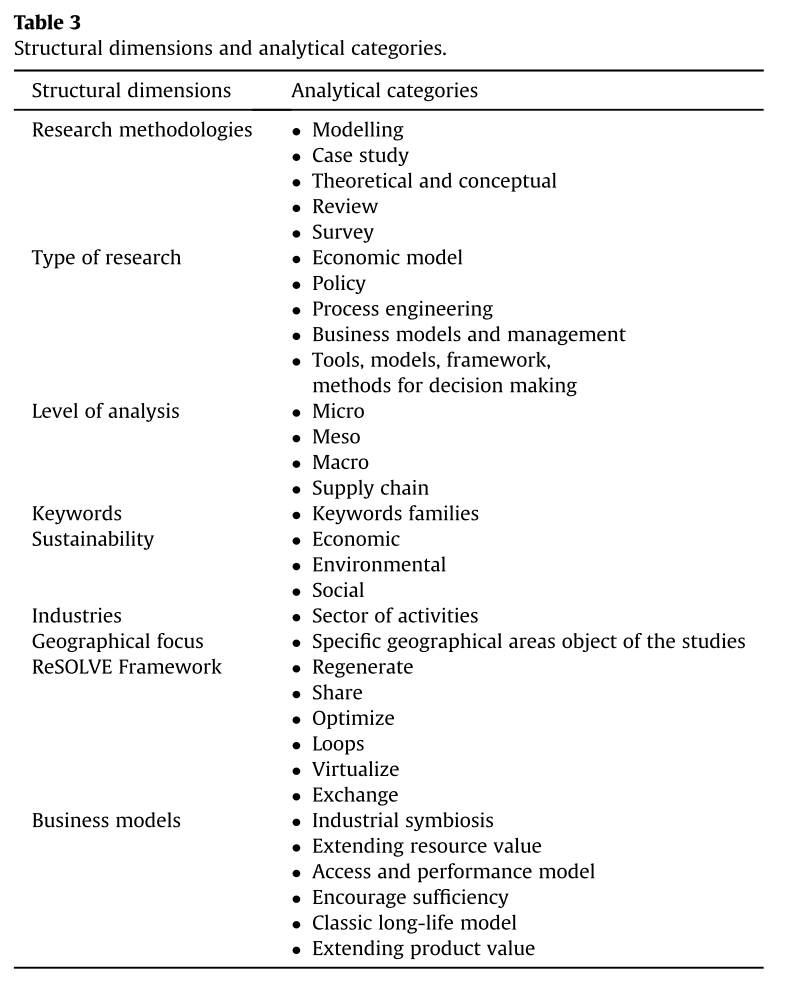
\includegraphics[width=0.6\textwidth]{sections/asset/cateogories of research.PNG}
    \caption{Categories of research}
    \label{fig:research cat}
\end{figure}

Regarding the different research methodologies, as analytical tools this research will be focusing on building conceptual frameworks, that can be used to model and take case studies to test the models. This means, that the type of research that will be engaged in this project will be aimed to develop tools, models, framework and/or methods for decision making. \par

Since the objective is to develop a general model to capture how waste flows in city-regions, this automatically means that the levels of analysis and scale of the project will be somewhere between a meso and macro level. Here individual choices or behavioral characteristics will be not be explored. \par
Finally, it will be focus on waste exchanges of different kinds, trying to understand to what extent the location of socio-economic activities affect the level of Circular Economy practices. 




\section{Circular Economy}

The research on CE is still at early stages and the role of location socio-economic activities within it needs to be further researched. As UN, EU and other governments as China, Singapore, Japan or The Netherlands, to name a few, make efforts to transition towards circular economy models, the paradigm/concept has expanded to city planning (Circular Cities, XXXXXX). Among the different circular economy strategies, in solid waste management and industrial symbiosis there are geographical elements to be considered and consequently of relevance for spatial planning agencies.\par

In this exploratory research project these different CE strategies will be approached with different objectives and methods; hoping that by making contributions and reflecting on these individual fields a more general statement about the relevance of planning can be made.\par

Dealing with IS and SWM, automatically creates another exclusion in the concept of CE. As the concept of CE could be found rooted as a spin of the 3Rs strategy to reduce the amount of waste produced (Reduce-Reuse-Recycle). Since its first appearance the idea of 3Rs has evolved and more Rs and other letters have been added to the main idea. Currently, the concept has crystallized into a 6 stages pyramid and this work will focus in the 2 stages of it: recycle waste, reuse waste. \par



\section{Geographical considerations}
Because of the geographical nature of Circular Economy, the work will be focused on SWM and IS and these systems cannot be contained to cities administrative boundaries \parencite{Dupuy2008}. The production of waste resources and it’s treatment are scattered across the territory, with interactions across municipalities and in some cases regions, thus require to take a more holistic and comprehensive approach. \par
Although, the exploration of theses strategies could be done under different scales; starting from an individual stakeholder, moving upwards in scale to a group, a neighbourhood a city and the system of cities that comprehend the system, in order to comprehend how sustainable the system is, it's important to take into consideration not only one unit but the whole network of cities that create a functional area.\par 




\section{Approach/Methodological}
The work developed during this project will be quantitative and embraces the Smart Cities movement. The work will benefit from advances in computer science, new sources of information and urban analytics. This delimitation is important because it defines the lenses and toolkit used to analyze the problem of waste materials in city regions. \par
The planning tools and frameworks of this works, need to be digital and with the capacity of capturing in a quantitative matter the dynamics of the system.\par
Moreover, an open-source and full transparency approach will be also adopted. This is an important condition of the present work because it will allow other researchers and practitioners to understand the tool box to be developed, but also by adopting this paradigm it allows the project to continue after it finishes. Everyone interested in improving or correcting these developments will be able to do it.  


\section{Other research delimitation}
Arguably, Circular Economy can be considered the next new paradigm that will contribute to materialize sustainable development. In order to qualify as such, the contribution to the three main sustainable development domains (Economically, Social \& Environmental) should become clearer. %(xxxxxxx). 
Research on CE is still in its infant stages and the concept is found contested.  %(XXXXX). 
Variations in its definition makes it difficult to implement creating gaps between theory and practice. \par %(XXXXXXX). \par

In this work, CE is understood as a set of strategies that eventually could became a new socio-economic regime but the contributions of ce to promote social justice are still unexplored. Moreover, issues related to institutions, politics or even behavioral changes such as trust or citizen involvement are out of the scope of the dissertation.\par
Finally, but not least important it is important to state that within the field of IS there is a an already well-developed corpus of research that focuses in Eco-Industrial Parks (EIP), which are co-located firms in pre-determined zone. Usually in these types of industrial developments, there is a natural tendency to reduce energy, water and other resources. Also, as a result of lower barriers IS arriving to higher stages of development: knowledge exchanges and other forms of co-operation. \par



\section{Case Studies}
Finally, the general framework and data model developed during this project are going to be tested by applying it to different context. For it, data availability will be crucial. This will require to establish relationships with different stakeholders and to begin a collaboration process. Currently, there are some potential institutions to collaborate with that work in the following places:
\begin{enumerate}
    \item CEAMSE - Buenos Aires Metropolitan Area
    \item WET - Sweden
    \item Metabolic - Netherlands
\end{enumerate}




%\section{Summary}

%This is an exploratory dissertation that will be trying to make a quantitative contribution to understand how space can be taken into consideration to enhance circular economy practices. In order to do so, among the different strategies 




%%%%%%%%%%%%%%%%%%%%%%%%%%%%%%%%%%%%%%%%%%%%%%%%%%%%
\chapter{Research Methodology and Description}
%%%%%%%%%%%%%%%%%%%%%%%%%%%%%%%%%%%%%%%%%%%%%%%%%%%%
The work packages of this project are detailed in this chapter. After breaking down the main research question into smaller and different components, in this section those components are going to be allocated into different stages. Some of these stages will be linked one to the other but, some of them will be executed simultaneously. The last stage of the research will collect the main learning from the other stages and contribute to the field in a more holistic way. All the other previous stages, will remain focal to a specific issue or knowledge gap within the waste material domain. As this research progresses and the last stage gains importance, the research will engage more in the main research question.

\begin{figure}[h!]
    \centering
    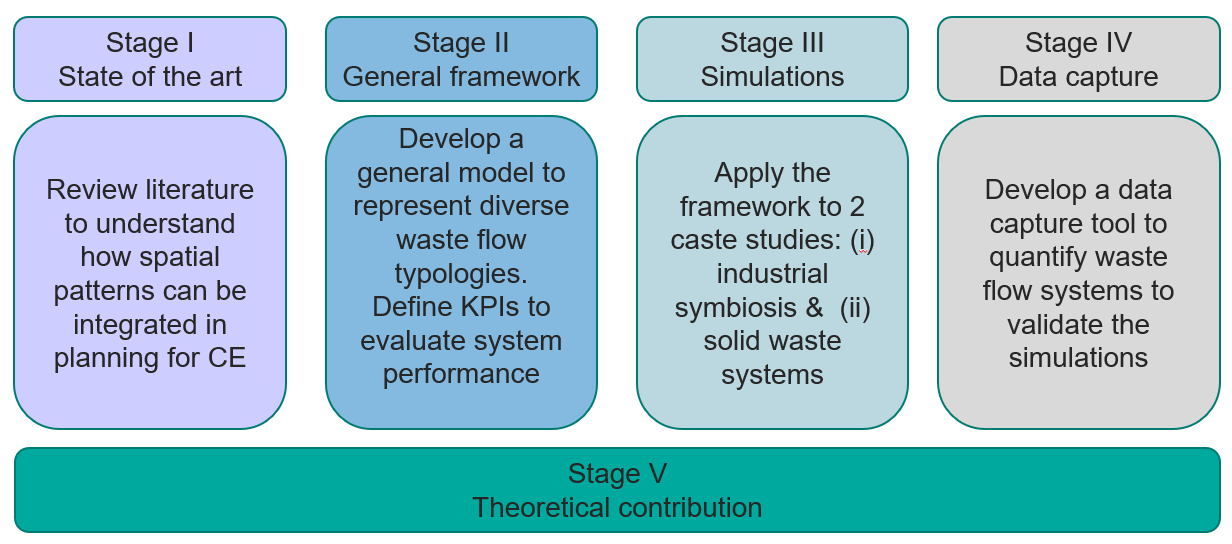
\includegraphics[width=0.8\textwidth]{sections/asset/stage.PNG}
    \caption{Details of stages of research}
    \label{fig:research1s}
\end{figure}

% -	This project is composed by 4 main sequential components and an optional 5th part, that will only be included if there is space to pursue it or it becomes clear that is a critical part of the project. \par
% -	In what follows in this section, I will be describe in greater detail the activities that will be executed in each component and how these components are connected to each other. \par
% -	These components were identified as necessary components to bring unambiguous answers to the main research question faced in this project.  \par
% -	This main question will eventually find partial solution at the end of this project and all the throughout the project different knowledge blocks will be built to reach to these objectives. \par
% -	Based on the identify problem and knowledge gap, the first main objective is to develop a data model capable of modelling how resources flow in a city region. \par
% -	Only then, it would be able to scrutinize the role of the location in closing the loop of resources. v
% -	The rest of this section describes in greater detail each of these four components. \par

\section{Stages of research}
The research has been divided 5 stages, of which 4 of them contribute to feed a fifth stage, that ultimately will use the main learning's from the previous stages. In this last stage the main research question will be addressed and where the main theoretical contributions will be made. During the first stage of the research mainly a literature review will be conducted. Once the marginal curve of leaning starts to flatten work towards a general framework of waste fluxes will start. As the general framework starts too become more stable and there is more certainty that it could be used for simulating different scenarios, the development of these scenarios will start. In parallel to this stage data structures are going to be explored and potentially collected. After the simulation and data capture stages are completed, the model of waste flows will be explored to further understand the role of location patterns to enhance circular economy at different geographical scales. 



In order to further comprehend how these stages relate to each other and how this research is going to progress see the diagram and the subsections below.

\begin{figure}[h!]
    \centering
    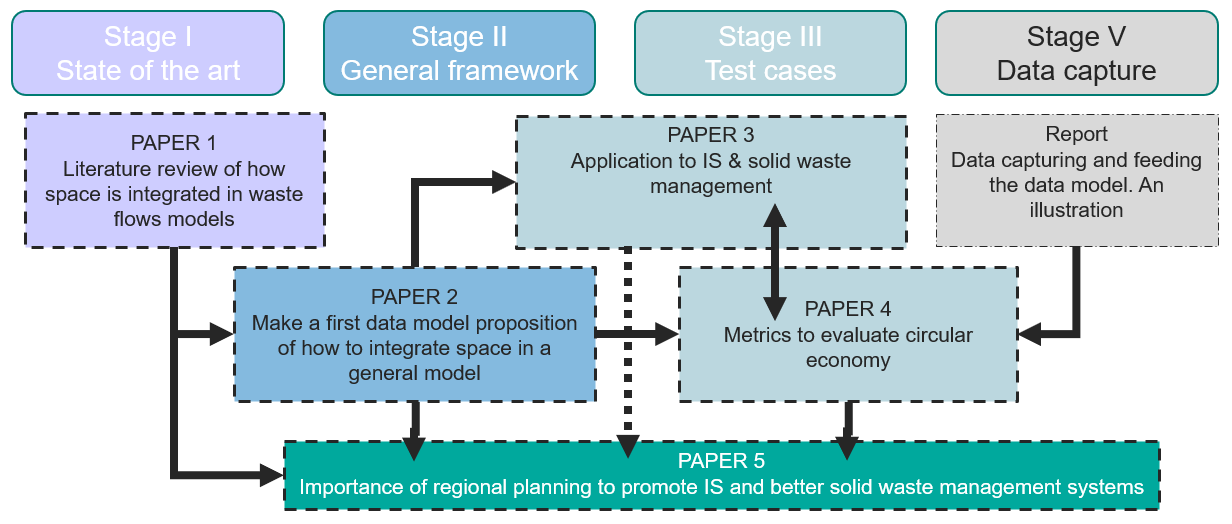
\includegraphics[width=0.8\textwidth]{sections/asset/stage2.PNG}
    \caption{Stages of research, interactions and outputs}
    \label{fig:research2}
\end{figure}






\subsection{Stage 1: Status-quo of modelling waste flows and measuring progress in circular economy processes}
The first stage of the project consists in gaining a better understanding of the concepts of circular economy, urban metabolism, industrial ecology (symbiosis) and municipal solid waste. After gaining more knowledge in these main fields, more specific exploration will be conducted to understand how space (location of socioeconomic activities) has been taken into account to describe and evaluate circular economy performance in city-regions. \par
In this case the objective is to comprehend to what extent space has been integrated into urban metabolism and circular economy ideas. Since one of the distinct attributes of cities and regions, is that these entities are spatial (as geographical), to describe them and to evaluate their performance space must be also considered.  \par
The output of the stage will be to reflect critically about sustainability, planning, circular economy, smart cities and other major concepts that will be referenced in this project. More specific, after the readings, it will become much more clear how space has been used to evaluate circular economy practices in the urban and regional domains. In order to tackle this tasks, an annotated bibliography will be written to highlight and pick major advances in these fields. \par
For this stage, Google Scholars, Scopus and Web of Science will be used to create a database of references to be studied and analyzed. This stage finishes with a deliverable that will be a publishable review that will highlight the need to incorporate space into these domains.\par



% •	Other deliverables: \par

% \begin{enumerate}
%     \item Table with circular economy metrics that take into consideration space 
%     \item Table of waste flow models that consider space
%     \item Simulations and models of waste flows
%     \item Stakeholders
%     \item Potential data providers 
%     \item Set of case studies
%     \item Important parameters
% \end{enumerate}


•	Research questions: 1.1 - 1.2 - 1.3    


\subsection{Stage 2: Design \& development of general framework the flow of secondary resources (waste)}
Towards the end of the second stage, it will be become more clearer how spatial patterns of activities have been modelled and taken into consideration to describe these urban systems. Moreover it will become clearer to what extent the location of activities has been taken into account to evaluate progress in circular economy.
Once it becomes clear how space has been taken into account in previous studies a general framework to study waste fluxes will be proposed.\par
This is a core part of the research since in order to study under a quantitative perspective the role of space and consequently the role of urban (and regional) planning, an operational framework would be needed. This framework will need to be prepared so that is could be populated with case studies and system properties. Open source and transparency of the framework are and performance will be studied. This part of the research requires the part above to be finalized and consequently it would be the point of departure to build the data model that will help up to represent how waste resources (secondary resources) flow in a city-region.\par
Departing from the knowledge gain from the previous stage during this stage a proto-model or conceptual framework will be developed. In order to do this, a clear map of the agents, its properties, how they relate and their action sets should be stated. Once this architecture is defined, the next step is to digitize on one hand the dynamic model, but also a relational data base, so that different case studies could be populated and evaluated. After the proto-model and conceptual framework become stable, this concepts will be digitized using R/PYTHON or a ABM Platform such as Eclipse or Net Logo\par
This stage is a core one, and it is expected that after completion two papers are in condition of being published. It is expected an article that shows the conceptual framework and proto-model comparing different waste cases and indicating potential uses. \par
•	Research question: 2.1 - 2.3 \par


\subsection{Stage 3: Test framework to evaluate solid waste management and Industrial symbiosis}
The conceptual framework is digitized and ready to be tested using different applications. These applications are case studies in different geographical areas and dealing with solid waste management and industrial symbiosis. The specificity of these case studies will depend on the data available for use. These case studies or applications will be used to populate the model. In this stage the model usefulness will be tested. By using the framework with these two waste systems the framework generality and usability will be stressed. As the model is being used and evaluated, there might be a need to change or re-think parts of the model. There will be interactions between this stage and the previous one.  \par
In order to progress in this stage, simulations and data acquisition of industrial symbiosis and solid waste management will be needed. Process the information so that can be integrated in the framework developed in the previous stage. Describe the system properties and evaluate how it is performing based on a set of KPIs. Define a set of scenarios to be modelled. \par
•	Research question: 1.2 - 2.1 - 2.3           \par

\subsection{Stage 4: Data capture and analysis to quantify and map solid waste generation}
This stage will be characterized by using existing data or developing methods to capture information about specific waste materials. By designing, developing or implementing a method to capture and analyze existing data about generation of waste it will be possible to produce tools to be used by practitioners. This will allow municipalities, collection services and recycling facilities to use this information to enhance the provision of those services.      \par
•	Research question: 3.1           \par



\subsection{Stage 5: Theory building, understanding the contribution of spatial planning to promote circular economy practices}
Finally, progress about metrics, models and data will allow to better understand how space determines Circular Economy practices. By combining these leanings, urban and regional planning tools could be used as a tool to promote Circular Economy practices a set of scenarios will be constructed for the two case studies. The idea of scenarios is intrinsic in planning practice and to elucidate what changes in spatial patterns should be promoted, consequently should be  important to run different scenarios and test different hypothesis. \par
This last stage of the research will be conceptual and it will be mainly aimed to contribute to build theory to bridge between urban and regional planning and environmental sciences. This publication would be pursued, only once the previous stages of the research are completed and only then, with the evidence of this project, attempt to bring some answers to general question that this project is trying to reveal. \par
•	Research question: 4.1 - 4.2 - General research question        \par
























% %%%%%%%%%%%%%%%%%%%%%%%%%%%%%%%%%%%%%%%%%%%%%%%%%%%%
% \chapter{Research Methodology and Description}
% %%%%%%%%%%%%%%%%%%%%%%%%%%%%%%%%%%%%%%%%%%%%%%%%%%%%
% This section details the specific methods and materials that will used in order to bring answers to the sub questions stated above. It is expected that by isolating these questions and answer them, an answer to the general research question will emerge. Taking as a starting point, an specific methodological tool set are selected. \par

% For each question try to fill the following form:

% %\textbf{\begin{itemize}
% %    \item Related Literature
% %    \item Data Set
% %    \item Methodology
% %    \item Plan
% %    \item Expected results 
% %\end{itemize}}


% (each sub section should be a task)
% (here is more about tasks)
% (results)


% \section{ Some thoughts on tasks:}

% \textbf{Review to understand}
% -Describing the system, "mapping" it, including space.
% - Identifying and describing in more detail subsystems for further work: IS and household/municipal

% \textbf{Review to assess}
% - Assessing the performance of the waste system: KPIs
% - Assessing the performance potential of the system from a CE perspective: building resilience, characteristic that will predispose it to perform well.

%  \textbf{The data gap issue}
% - Data can be inferred/potentials estimated (see IS work); 
% - data can be simulated based on model of the system; 
% - data can be collected (based on data model): "manually" by actors, or digitally by systems.
% - some empirical data useful to calibrate/validate the simulation and the inferences.
% - real data is necessary for calculating KPI

%  \textbf{The model}

% \textbf{The planning issue}
% - potential/inference/statistics/analysis is necessary for planning guidance towards KPI. What measures should one take with the limited resources and time? To examine the baseline and test scenarios. 



% \section{Metrics and key performance indicators}


% \begin{figure}[h!]
%     \centering
%     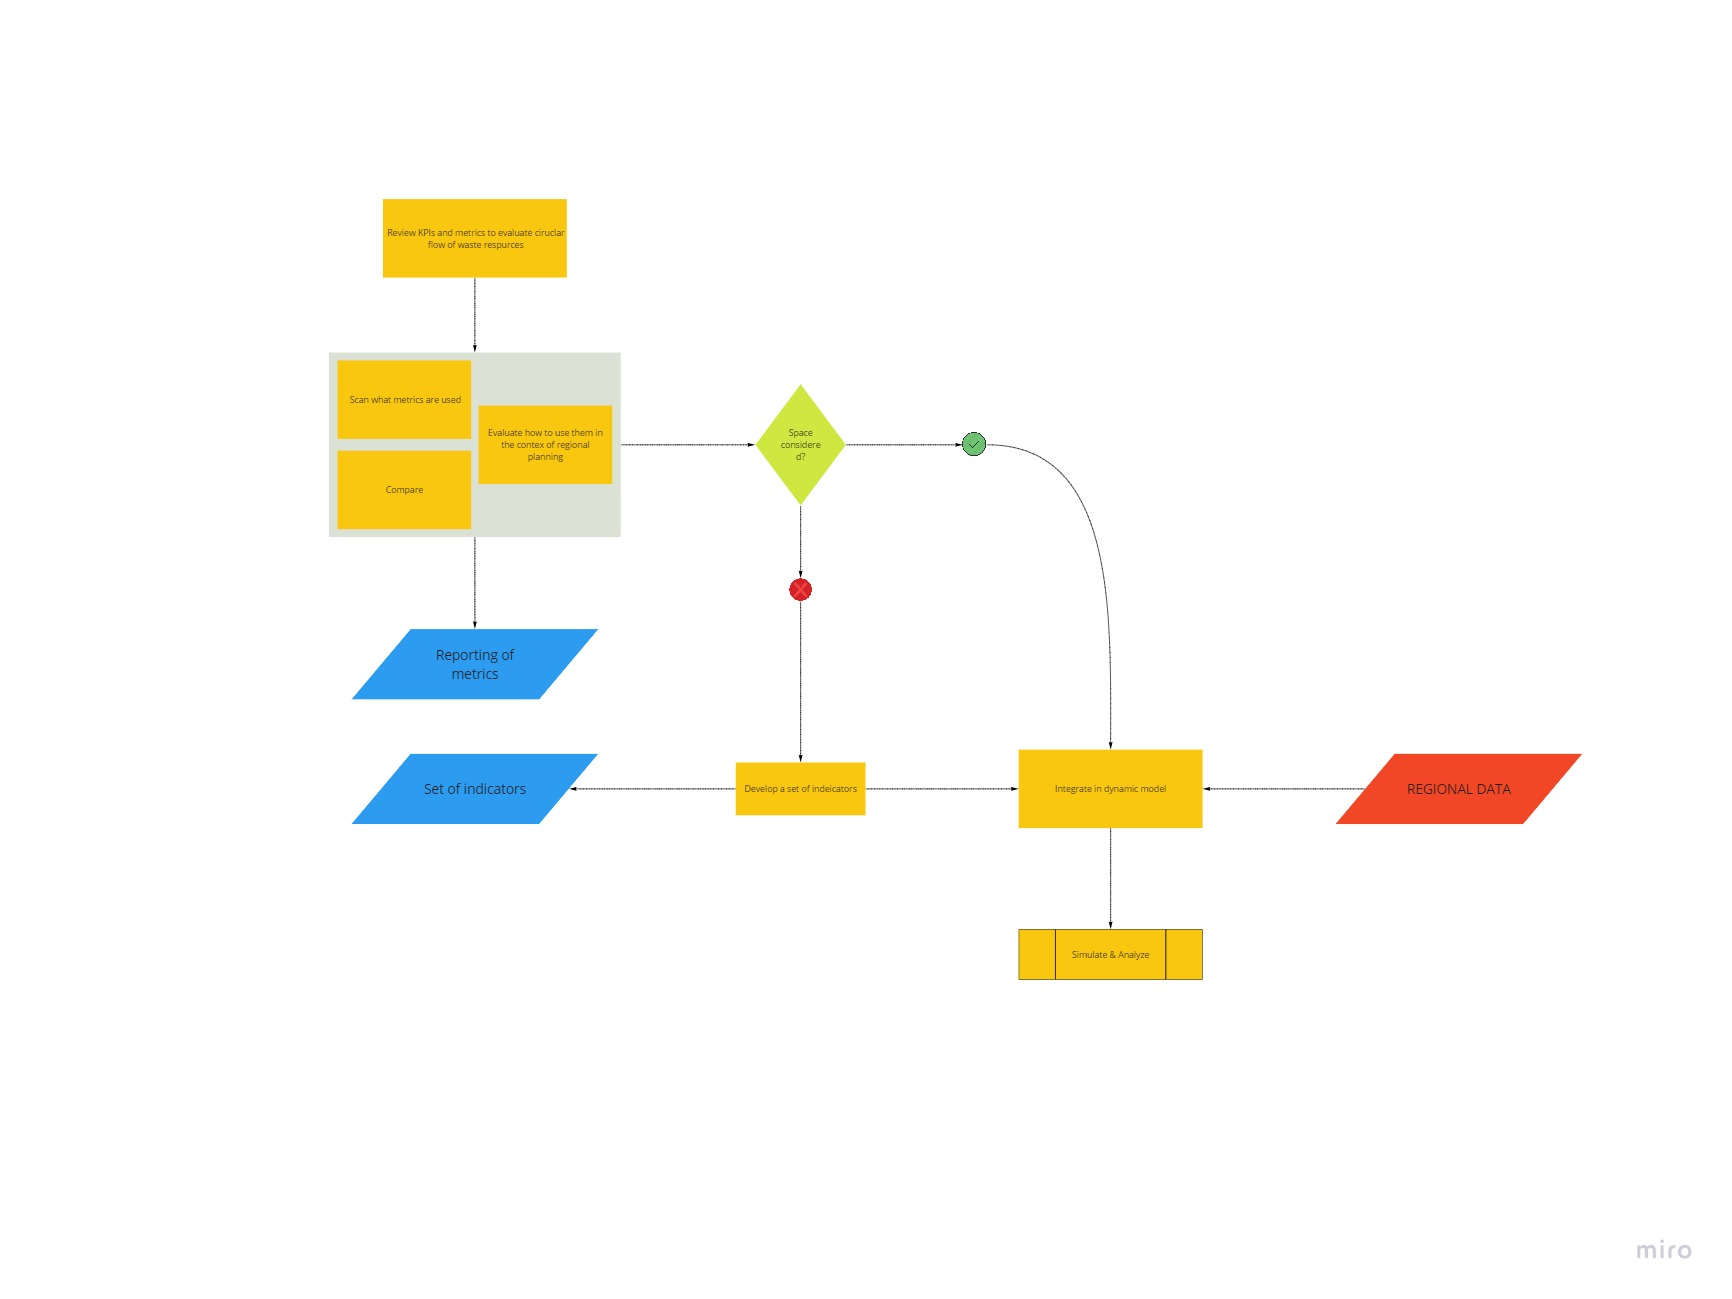
\includegraphics[width=0.8\textwidth]{sections/asset/PHD2 tasks - Metrics exploration.jpg}
%     \caption{Task and workflow for metrics exploration}
%     \label{fig:phd1}
% \end{figure}


% \subsection{State of the art}


% \subsection{Incorporate space into metrics}



% \subsection{Test metrics in models}


% \section{Data capture and processing}



% \begin{figure}[h!]
%     \centering
%     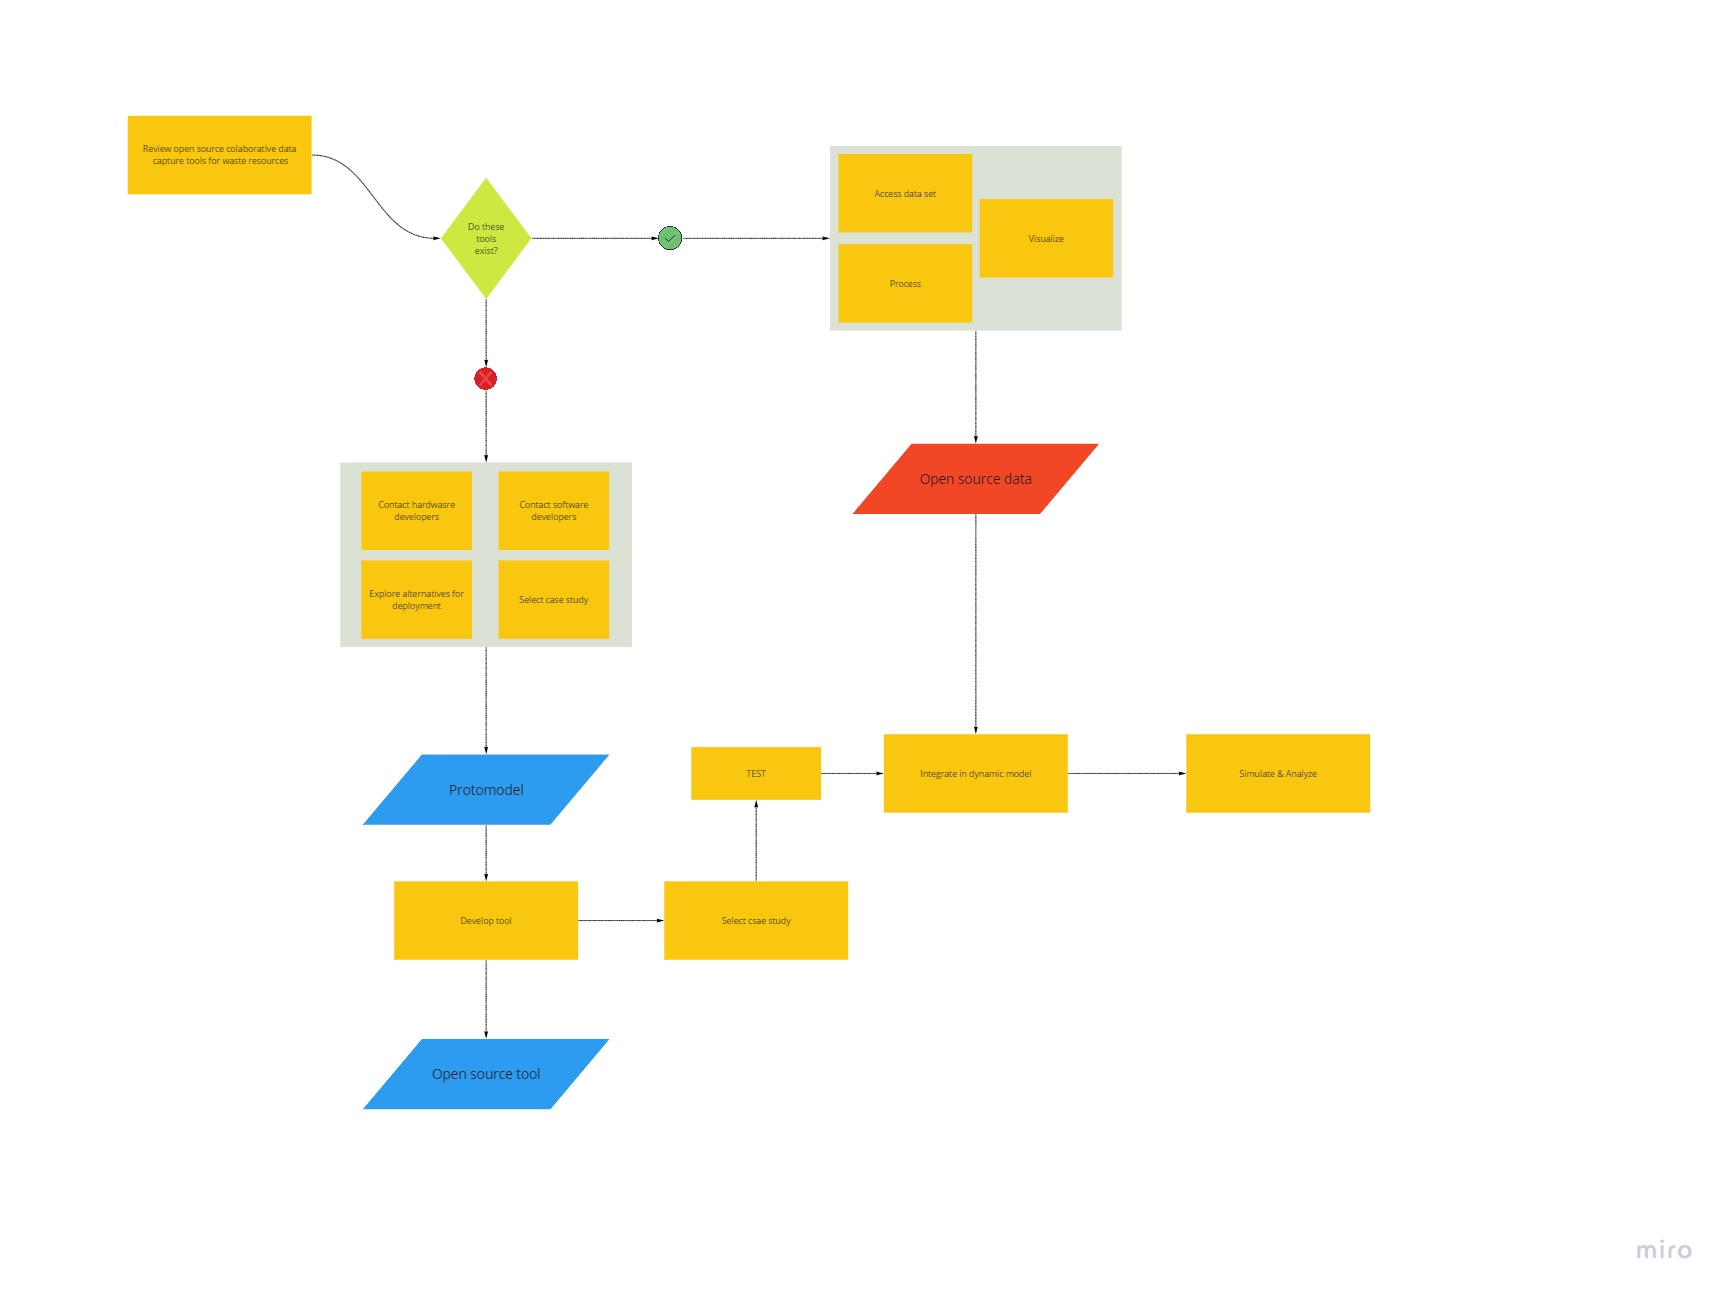
\includegraphics[width=0.8\textwidth]{sections/asset/PHD1 tasks - Data capturing workflow.jpg}
%     \caption{Task and workflow for metrics exploration}
%     \label{fig:phd2}
% \end{figure}
% \subsection{State of the art}

% \subsection{Feed a data model}


% \subsection{Analyze preliminary results and indicate future research}


% \section{Models}


% \begin{figure}[h!]
%     \centering
%     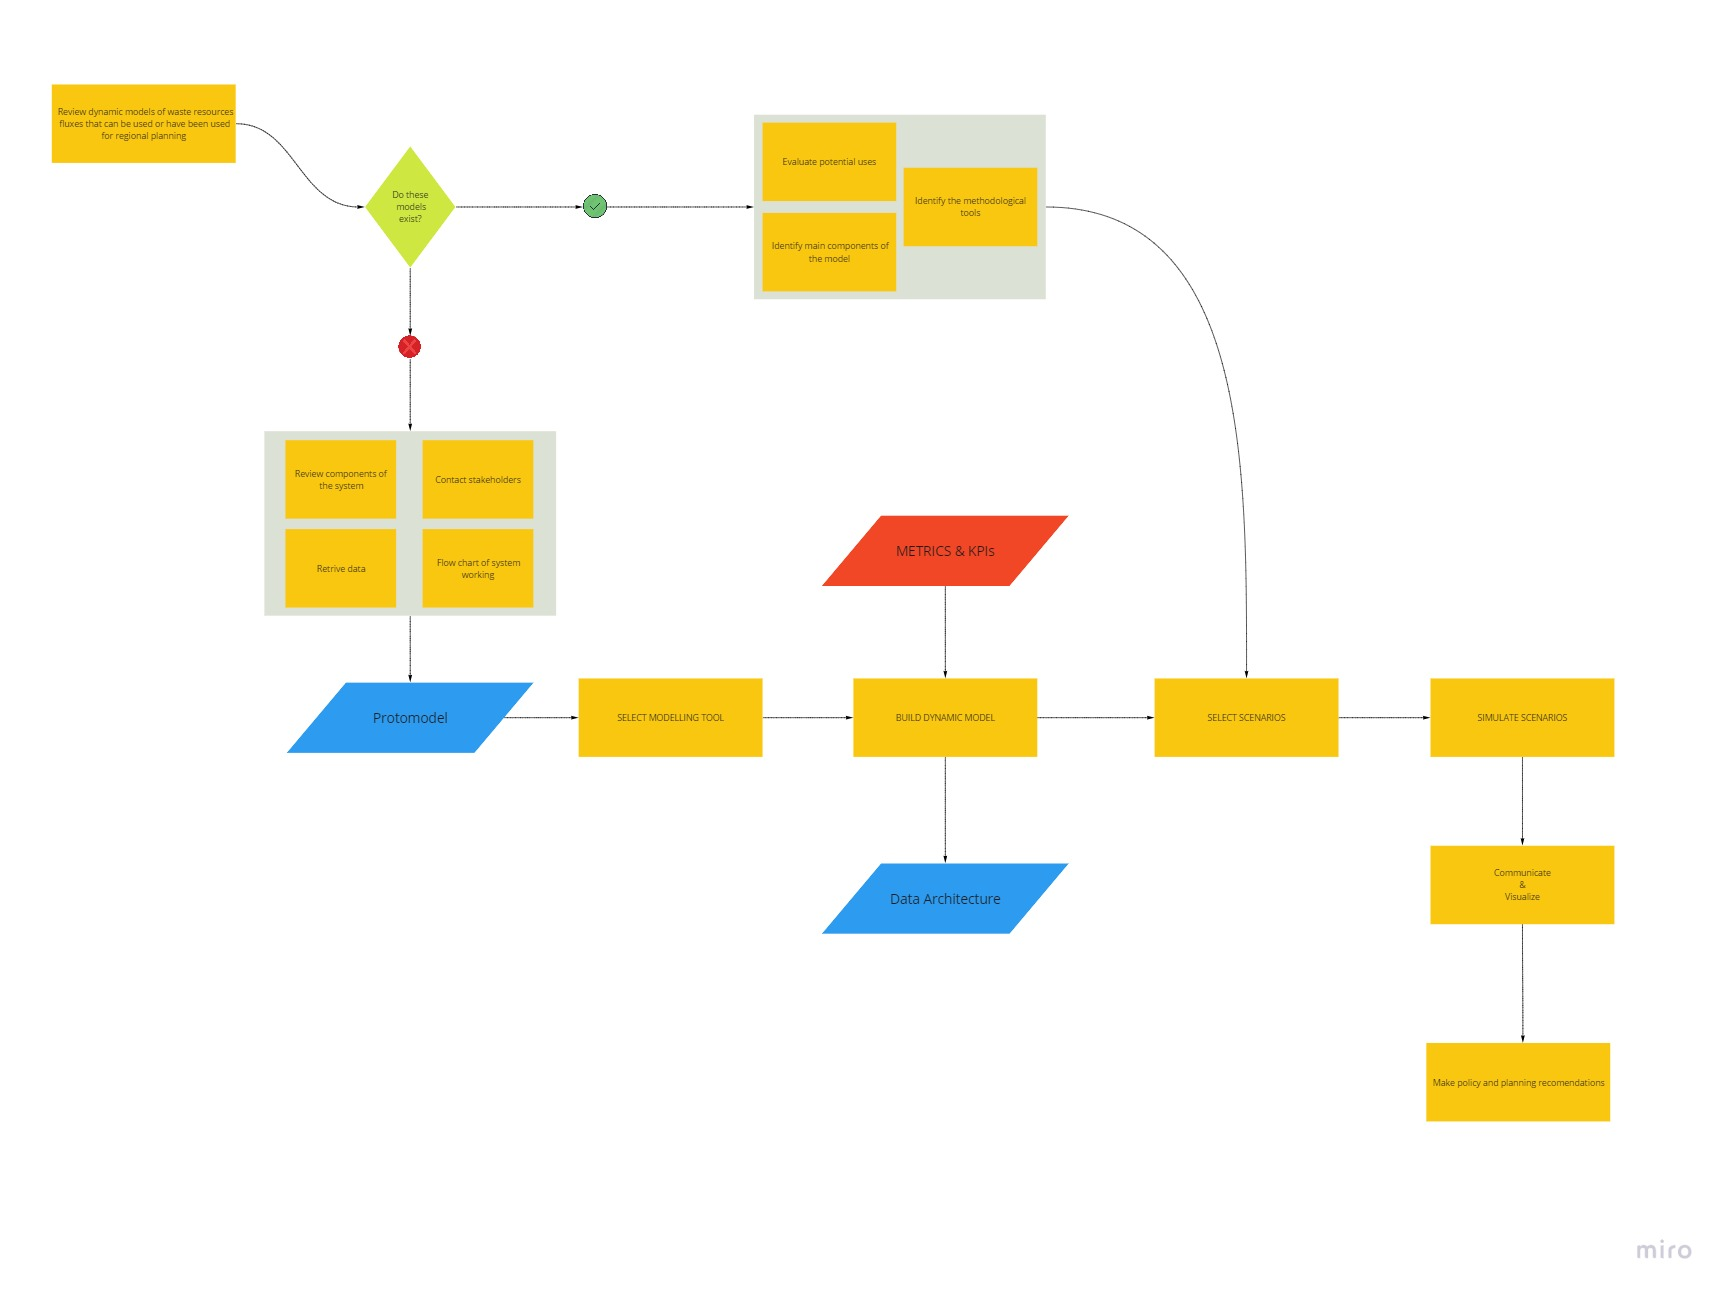
\includegraphics[width=0.8\textwidth]{sections/asset/PHD3 tasks - Modelling workflow.jpg}
%     \caption{Task and workflow for metrics exploration}
%     \label{fig:phd3}
% \end{figure}
% \subsection{State of the art}




% %%%%%%%%%%%%%%%%%%%%%%%%%%%%%%%%%%%%%%%%%%%%%%%%%%%%
% \section{How is the flow of waste resources in a city-region being assessed and what key performance indicators are calculated in order to evaluate how sustainable waste materials flow in a region?}\par
% %%%%%%%%%%%%%%%%%%%%%%%%%%%%%%%%%%%%%%%%%%%%%%%%%%%%

% The aim of this component is to explore the literature of Industrial Symbiosis in search for regional indicators that capture the environmental performance. As seen in the problem definition, in the field of Industrial Symbiosis, space have been omitted and instead a-spacial material flow diagrams have been used to describe the performance of industrial exchanges.  \par

% For this component a literature review will be pursed to better understand how space and urban planning have been addressing the use of waste materials and what key performance indicators should be taken into account to design healthier regions?\par

% In this case, the underlying hypothesis is that space, the specific location of economic activities have not been adequately addressed in the field of Industrial Symbiosis and consequently, the Key Performance Indicators are not suitable to inform regional design practices. \par

% As a result, this component will extract what is the current state of the art to evaluate how sustainable waste resources are flowing in a city-region.\par 

% %%%%%%%%%%%%%%%%%%%%%%%%%%%%%%%%%%%%%%%%%%%%%%%%%%%%
% \section{What can be learn by reviewing well documented case studies? How would a model that captures the flow of waste materials in a region should look like?} \par
% %%%%%%%%%%%%%%%%%%%%%%%%%%%%%%%%%%%%%%%%%%%%%%%%%%%%


% What information is currently being captured? How is space incorporated in these assessments? What role does it play?\par
% Do conclusions drawn from a-spatial material flow diagrams are still valid if space and the costs of moving residual material are taken into account?

% The aim of this component is to review the existing literature of Industrial symbiosis to capture what key performance indicators are being measured and, if the location of firms - space -, is taken into consideration, what role does it play. Given that the domain of Industrial Symbiosis have been focusing on the flow materials, space and the location of firms have not been taken into consideration. Different performance indicators have been developed to asses the performance of industrial symbiosis exchanges, Sbut still the geographical structure have not been fully incorporated. The lack of desegregated information about individual firms, and the fact that the field of Industrial Symbiosis is heavily rooted/associated with Eco-Industrial Parks, where by construction, all firms are co-located, space has not been perceived as a variable to be taken into consideration. \par 
% In this component, this fact will be exposed by looking at how other researcher have been measuring the performance of Industrial Symbiotic relationships. By incorporating space and costs, adding more complexity can introduce conflicting objectives. 


% %%%%%%%%%%%%%%%%%%%%%%%%%%%%%%%%%%%%%%%%%%%%%%%%%%%%
% \section{How can waste material exchanges between industries in a region be spatially modelled? what key performance indicators can be developed using this model?}\par
% %%%%%%%%%%%%%%%%%%%%%%%%%%%%%%%%%%%%%%%%%%%%%%%%%%%%

% Based on case studies of existing industrial symbiosis and the data set of industrial symbiosis developed by the Urban Metabolism group at Chalmers, extract the main features and characteristics that describe the industrial exchange of waste resources. Using the information extracted, design the logic and the data structure of a model that can be used to capture these exchanges. \par

% To start with, using the location of industries, their material inputs and waste resources output, a geographical model will be developed and a set of performance indicators evaluated under different assumptions. \par

% One the structure of the model is settled, meaning that the attributes and the interrelations of the model are not still changing, the model will then be transferred to an agent-based environment where different fluxes will be simulated to study how the performance indicators change as the parameters of the model exchange.
% The expected result of such a description, will be a platform that allows to model and measure different aspects of industrial symbiosis and asses the performance of different scenarios of exchange.\par

% %%%%%%%%%%%%%%%%%%%%%%%%%%%%%%%%%%%%%%%%%%%%%%%%%%%%
% \section{How should waste materials flow in a region in order to achieve an optimal resource usage? How much would it cost to achieve an optimal flow of waste material at a regional level?}\par
% %%%%%%%%%%%%%%%%%%%%%%%%%%%%%%%%%%%%%%%%%%%%%%%%%%%%
% This question is a theoretical own and the aim here is to develop a best case scenario that will help to benchmark the current situation of the regional exchanges of waste materials. Given, the lack of information about the current state, in this case and Agent Based Model will be explored to simulate possible solutions for industrial symbiosis. Different scenarios will show how to optimise for different key performance indicators.\par

% In order to model regional exchanges of waste resources, SEB data set of firms will be explored. Using some of the knowledge building blocks developed by the group of Water Environment Technology at Chalmers, waste by-product types and quantities will be used. An agent-based modeled will be developed to simulate different combinations of material exchanges. The simulations will track different key performance indicators and solutions that maximise them will be computed. This scenario builder will contribute as a benchmark to what is actually occurring in the territory. \par

% This benchmark will allow regional plans to find a direction to steer their regional policies. 
% As a by-product of this research, the exploration of these solutions will contribute to understand possible conflicts between different objective functions. For instance, Co2 emissions caused by transporting the waste resources to its optimal place of use might be higher than disposing it to the nearest treatment facility. \par

% Finally, but not least by modelling scenarios for different objective functions, the cost for different scenarios can be modelled.\par 

% %%%%%%%%%%%%%%%%%%%%%%%%%%%%%%%%%%%%%%%%%%%%%%%%%%%%
% \section{What are the potential uses of such a model? Can this model structure be also used to model the waste at a city level generated by households and managed by a municipality?}\par
% %%%%%%%%%%%%%%%%%%%%%%%%%%%%%%%%%%%%%%%%%%%%%%%%%%%%
% The aim of this component is to continue exploring the model developed above and exploit it  to understand what if scenarios. The model should be open to modify the location of industries, or locate new facilities. As these modifications are incorporated, it is expected that waste exchanges dynamics will change and eventually have impacts on the performance indicators. \par
% By making these modifications to the current information, hypothetical scenarios contribute to transform the tool into a regional planning tool, that will allow practitioners or policy makers to understand how different spatial configurations perform different. 


% %%%%%%%%%%%%%%%%%%%%%%%%%%%%%%%%%%%%%%%%%%%%%%%%%%%%
% \section{Residential solid waste generation and management}\par
% %%%%%%%%%%%%%%%%%%%%%%%%%%%%%%%%%%%%%%%%%%%%%%%%%%%%

% These components, 
% %%%%%%%%%%%%%%%%%%%%%%%%%%%%%%%%%%%%%%%%%%%%%%%%%%%%
% \subsection{Does waste sorting and collaboration with urban recyclers improve the efficiency of urban solid waste management systems}\par
% %%%%%%%%%%%%%%%%%%%%%%%%%%%%%%%%%%%%%%%%%%%%%%%%%%%%




% %%%%%%%%%%%%%%%%%%%%%%%%%%%%%%%%%%%%%%%%%%%%%%%%%%%%
% \section{How to capture information about the amount and quality of waste generated in residential zones?}\par
% %%%%%%%%%%%%%%%%%%%%%%%%%%%%%%%%%%%%%%%%%%%%%%%%%%%%

% The aim of this component is to develop and open source tool to quantity and characterise waste generated by households. By developing a smart bin and providing an specific data feed pipeline, individual household data can be collected, aggregated and processed to inform the waste collection system.
% Moreover it will contribute to provide a systematic methodology of measuring waste, using a smart bin will guaranty that the information is collected in a systematic way IoT will allow to create a network of connected bins that will produce valuable information to enhance waste management capacities. 


% %%%%%%%%%%%%%%%%%%%%%%%%%%%%%%%%%%%%%%%%%%%%%%%%%%%%
% \section{What methods can be used to capture information about the activity of informal recyclers in the context of the global south?}\par


% %%%%%%%%%%%%%%%%%%%%%%%%%%%%%%%%%%%%%%%%%%%%%%%%%%%%
% \section{How can information of collection and generation be integrated and used to enhance the operation of the solid waste management system}\par
% %%%%%%%%%%%%%%%%%%%%%%%%%%%%%%%%%%%%%%%%%%%%%%%%%%%%


% %%%%%%%%%%%%%%%%%%%%%%%%%%%%%%%%%%%%%%%%%%%%%%%%%%%%
% \section{Data model}\par
% \subsubsection{To what extent the industrial symbiosis and residential solid waste system can be captured using the same data model?}\par
% %%%%%%%%%%%%%%%%%%%%%%%%%%%%%%%%%%%%%%%%%%%%%%%%%%%%

\chapter{Research plan}
In order to achieve the research and educational objectives of this project, in this chapter the expected time line to be followed, the list of planned publications and the list of courses to attend are presented. 



\section{Time plan}
The time line below shows the set of activities to be pursued during the project and when they will be happening. The time line shows that some of the activities in the project are needed to be executed in parallel and some other require inputs from previous stages to be completed. The second part of the table shows what are academic articles to be delivered as the project progresses. \par
Following the stages above, during the first year the domain of research and the research questions were defined. This was possible as a result of background readings on different fields and realizing a knowledge gap a need from policy makers and practitioners to spatialize the concepts of circular economy. The second year will be focused on developing a general framework and data model that will allow in the follow up stages of the research to evaluate scenarios, describe an urban system in terms of waste management (municipal or industrial) and study its performance. 
The table below details the tasks that will be executed in the future. \par

\begin{figure}[h!]
    \centering
    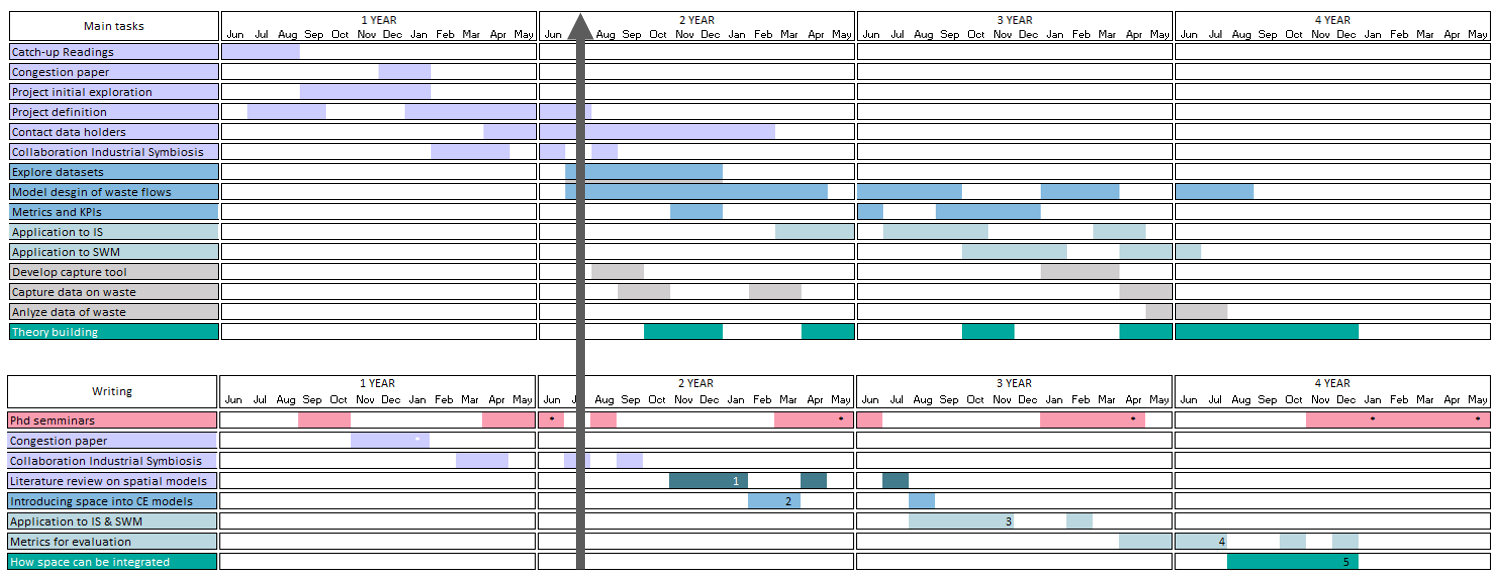
\includegraphics[width=0.95\textwidth]{sections/asset/timeplan.PNG}
    \caption{Time plan for the research proposal}
    \label{fig:research_time}
\end{figure}


The second part of the diagram shows what stages will be related to what publications. This is the list of publications suggested: 



\subsubsection{2020. Literature review of how space is integrated in waste flows models}


\subsubsection{2020. Make a first data model proposition of how to integrate space in a general model}


\subsubsection{2021. Application to IS \& solid waste management}


\subsubsection{2021. Metrics to evaluate circular economy}


\subsubsection{2022. Importance of regional planning to promote IS and better solid waste management systems}


\subsubsection{2022. Data capturing and feeding the data model. An illustration} 



% \section{Deliverable}



% \section{Doctoral education}

% \subsection{GTS - Mandatory}

% \begin{enumerate}
%     \item [DONE] Sustainable development: values, technology in society, and the researcher GFOK105 • 3 HEC
%     \item [DONE] General introduction for doctoral students GFOK015 • 0 HEC
%     \item [DONE] Career planning - your personal leadership GFOK010 • 1,5 HEC
%     \item [After Lic] Teaching, learning and evaluation GFOK020 • 3 HEC
%     \item [After Lic] Popular science presentation GFOK070 • 0 HEC
% \end{enumerate}

% \subsection{GTS}

% %\begin{enumerate}
% %    \item 
% %\end{enumerate}

% \subsection{Topic specific}

% \begin{enumerate}
%     \item Urban Metabolism \& resources
%     \item Industrial Ecology
%     \item 
% \end{enumerate}








\chapter{Preliminary results}
Here the activities and results from the first year activities are registered. This section details the contacts established, projects and conferences 



\section{Contacts and meetings}
A set of stakeholders and potential data holders were contacted for collaboration. Institutions and actors from the Netherlands, Sweden, Portugal and Argentina were contacted. Conversations with some of these actors will continue during the following months to improve the needs of practitioners and what information could be used to populate the data model. In the table below the status of the contacts is highlighted. 
\begin{figure}[h!]
    \centering
    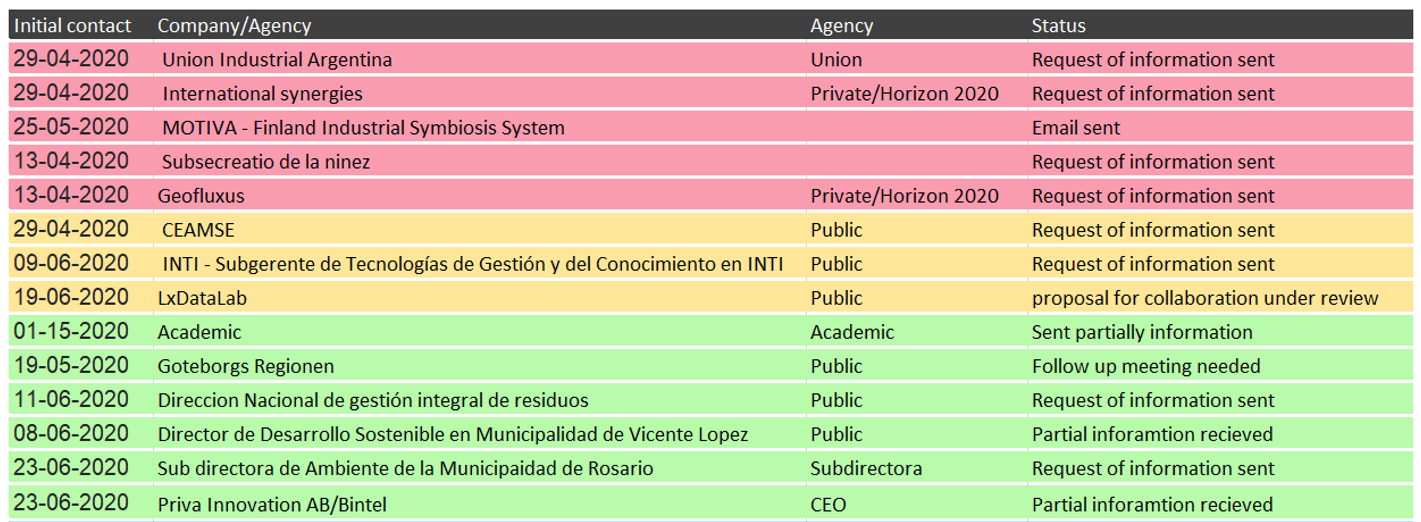
\includegraphics[width=0.95\textwidth]{sections/asset/contacts.PNG}
    \caption{Contacted stakeholders for collaboration}
    \label{fig:collaboration}
\end{figure}

The list of main potential partners are listed below:
\begin{enumerate}
    \item Dsposal (UK)
    \item Urban Metabolism group from WET at Chalmers (SWE)
    \item CEAMSE (ARG) 
\end{enumerate}


% \subsection{Household Waste}
% 13-04-2020: https://www.buenosaires.gob.ar/desarrollohumanoyhabitat/institucional-subsecretaria-de-ninez-y-adolescencia \par
% 29-04-2020: https://www.buenosaires.gob.ar/ciudadverde/separacion/porque-debemos-separar/programa-sello-giro\par
% 08-06-2020: Director de Desarrollo Sostenible en Municipalidad de Vicente Lopez \par

% \subsection{Industrial Associations contacted}
% 29-04-2020: https://www.uia.org.ar/medio-ambiente-y-desarrollo-sustentable/institucional/\par
% 29-04-2020: https://www.international-synergies.com/what-we-do/for-research/\par
% 29-04-2020: https://www.ceamse.gov.ar/generadores-privados/\par
% 05-05-2020: Informal data request to CEAMSEhttps://www.overleaf.com/project/5ea1c1fe57aac30001c2e0ec\par
% 25-05-2020: Marian Chertow\par
% 25-05-2020: MOTIVA - Finland Industrial Symbiosis System\par
% 08-06-2020: Director de Desarrollo Sostenible en Municipalidad de Vicente Lopez \par
% 09-06-2020: INTI - Subgerente de Tecnologías de Gestión y del Conocimiento en INTI \par
% 11-06-2020: Director de Desarrollo Sostenible en Municipalidad de Vicente Lopez \par
% 11-06-2020: Director de Desarrollo Sostenible en Municipalidad de Vicente Lopez \par
% 11-06-2020: CEAMSE \par
% 11-06-2020: Ex-director Nacional de gestión integral de residuos en el gobierno anterior: Luis Lehmann\par
% 19-06-2020: Subsecretaria de Ambiente de Rosario: Natalia Feldman\par

\section{Publications}

\subsubsection{A top-down method to support the identification of opportunities for Industrial Symbiosis partnerships}
Industrial Symbiosis (IS) can reduce industrial waste as well as the need for virgin material extraction by utilizing waste generated by one industry as raw material for another. Input-Output Matching is a commonly used method for identification of potential IS partnerships. In order to collect the data necessary to identify such opportunities, companies need to participate in activities such as workshops, surveys, or online questionnaires. However, these activities can be costly and time consuming. Additionally, companies may be unwilling to participate due to issues around data confidentiality. This article aims to show how these barriers can be overcome by a new method for identification of IS opportunities, which does not require companies to be surveyed. The developed matching approach makes use of statistical datasets and IS databases. The underlying principle is to use known IS partnerships and databases containing data on typical waste generation and resource use by industries to identify and link potential donors and receivers with similar characteristics, operating in other industry sectors. This allows expansion of a single IS case into multiple potential relationships. The method promotes Circular Economy development by finding ways to utilize more secondary resources through connecting previously unrelated industry sectors. The method has been tested in the Västra Götaland region in Sweden, where the goal was to identify potential partnerships between industries that generate sawdust as a waste product and companies that may be able to utilize this in their industrial processes. 159,630 of a total of 6,726,534 potential symbiotic links identified by the method were shortlisted, using prioritization criteria reflecting an increased likelihood of symbiosis.

\subsubsection{Mapping the spatial distribution of the effects of urban traffic congestion: methodological exploration using web based services}
Sustainable transport systems are a necessary requirement to achieve efficient economic performance, enhance urban quality of life and diminish environmental costs. Congestion, a negative externality of mobility, is responsible for urban pollution, inefficiency and has adverse effects over individuals facing this problem. For these reasons, transport and city planning agencies have developed interests in defining and measuring transportation congestion. Although, different definitions and metrics have been used, congestion measurements are found aggregated at a city level or for particular road segments. This study proposes a methodology that produces information from a web traffic service to map traffic congestion within an urban area. The method is simple and generalizable enough to be adopted in different urban areas. This paper presents the analysis of four European cities (Amsertdam, Glasgow, Goteborg and Lisbon) and show that the conclusions are consistent with the results obtained from internationally recognized organizations such as INRIX and TomTom.


\subsubsection{10\% Seminar \& report}




% \subsubsection{25\% Seminar \& report}


%\subsubsection{Annotated bibliography}



\section{Other research activities}
\subsubsection{Historical map of Gothenburg}
\href{https://chalmers.shinyapps.io/Goteborg_historical/?_ga=2.267750478.1104859035.1597823961-1745043960.1597823961}{Historical map of Gothenburg web site}


\subsubsection{Co-Design cards for Workshops in COVID-19 Times}

\href{https://chalmers.shinyapps.io/Goteborg_historical/?_ga=2.267750478.1104859035.1597823961-1745043960.1597823961}{Co-Design Cards}

\subsubsection{101 Lives - 48H Hackathon}
Hackathon aimed to propose strategies to reduce traffic accidents. I engaged in two teams that were awarded winners. The conversations with the insure company continued and they invited the team members to do a presentation to the company. 

\subsubsection{Economic Networks at Oxford}
In June 2019, the Economic Networks Summer School took place at oxford were a variety of advances in networks, tools and applications were introduced. 
\chapter{Self-Reflection}


It seems that without establishing a set of measurable goals, the New Urban Agenda will be hardly exercised \cite{Caprotti2017, Valencia2018}. Many other institutions ranging from NGOS, businesses, local authorities, or other international agencies also monitor different dimensions of urban life, but still, these indicators capture the output of a phenomena; not the process behind a specific result. Different urban variables are being monitored all the time, (i) in some case the variables may have direct connection to an SDG, such as levels of C02 emotions, (ii) the variable can be a property of the system, such as the total length in km of roads, or (iii) an indirect variable that correlates with the SDG indicator (CO2), for instance; congestion.  \par


Research on cities and urbanity is complex and interactions between different non-linear systems must be taken into account and as a result 
\begin{quote}We cannot predict future cities, but we can invent them. Cities are largely unpredictable because they are complex systems that are more like organisms than machines. Neither the laws of economics nor the laws of mechanics apply; cities are the product of countless individual and collective decisions that do not conform to any grand plan. They are the product of our inventions; they evolve. \parencite{Batty2013}\end{quote} 

After slowly accepting the nature of Planning Problems and the complexity of urbanity, I started to wander what is my role  as a researcher? and How would I like to position myself in the field? (What does it mean to 'do' science in this context?) \par 
In response to both enquiries I decided that as much as, and for as long as possible, I would like to stay away from the Issue Advocate role and mainly stay as a Pure Scientist that when required can contribute to answer specific policy questions by engaging as a Science Arbiter \cite{Brown2008}. \par
One of the advantages, of being at a such an early stage in my research is that, at some point, I can steer the direction of the research and having this in mind I started not to feel so comfortable with building simulations, predictive modelling or trying to solve a concrete urban challenges, such as gentrification. Instead, after much debating with my supervisor we decided we were going to start studying the characteristics of the waste and food systems. By describing parts of the system in greater detail, eventually the links between form, function and performance will be clearer. I believe that if we want to change the specific outputs or performance of a system it is imperative to first disclose its parts and the interaction within its pats and how they relate to other systems.  \par

In this sense my research could be contested at an intellectual plane, discuss to what extent my assumptions are valid ones. The output of the research will hopefully be used by policy makers and contribute to raise awareness of the degree of complexity of this issues. By doing so, I realize that I’m adopting a Precautionary principle, as actions or strategies should be carefully implemented. As wicked as they are, they could backfire and introduce an undesirable effect. 



\section{Ethics concerns around the smart city paradigm}
\subsection{On privacy issues}
Because an important part of my project will deal with exploring and developing new data sets from the ground by using public information and merging it with secondary granular data, at some point I might face some privacy issues.  To start with, there will be copy right issues and limitation on how a data can be handled. The second major data relates to Individual Privacy Rights and by collecting and merging some data systems, some effort should be allocated to debate the legal or ethical implications of these practices.  \par

In order to tackle some of these ethical, with my supervisor we agreed to work with open source software, to open the codes developed during this research project and to free the data created. Under our understanding, working under an open data agenda and collaborating with other institutions contributes to link the research to meet the SDGs. By promoting more transparent processes and interaction with different stakeholders, the science of cities can advance faster and start moving away from the Ivory Tower. \par

This is an assumption, a normative stand we have decided to make as researchers, and I should reflect much more on this issue. For instance, as debated during the lectures, should we open the data sets as soon as the research is done? Or should we wait to individually exhaust the opportunities of the dataset before we release it? Hopefully, when the times comes, the answers to these questions will still be to cooperate, open processes and data; while protecting privacy. \par


\subsection{On technological ubiquity}
Certainly, these new ‘bottom-up’ data sources have contributed to improve our understating of human settlements and in some cases enhance quality of life. As the ubiquity of internet, cellphones, computers, cameras and monitors became a fact we have witnessed the buzz for the Smart City. Academic communities, governments and businesses blinded by the infinite opportunities that mining these new data flow could produce, could not see (or decide to ignore) what George Orwell foresaw in his sci-fiction world. \par

This practice is not new, conscious or intentional; in a completely different context G. B. Shaw reflected on how doctors were assessing other doctor practices and concluded that: 'All professions are conspiracies against the laity' \cite{10.1093/ije/dyg233}. \par

When writing these lines, Shaw wanted to expose that there is a natural tendency of professionals in a same circle to cover themselves and avoid mutual criticisms. This reflection makes me wonder to what extent by using these new gadgets and data sets I am promoting and reinforcing the dynamics of technology ubiquity. If this is the case and I agree with some of the concerns raised against the smart city movement, then doing this research is challenging my beliefs and values of what urbanity should look like. \par

Slowly, as some negative consequences of adopting these consequences are becoming a reality, some academics, activists and institutions have started to rise concern with this new socio-technical regime. \par


%\subsection{On specific products and practices}


\subsection{Closing discussion}
All together, the development of this reflexive essay with the topics covered during the course helped me to raise awareness about my motives to purse a Phd in Urban Analytics. As the course progressed I was able to gain perspective over the context of my research and potential implications to different stakeholders. During these weeks I felt challenged and provoked to question my research and the possible consequences of it. \par 

Besides the concepts around ethics and sustainability, one of the most valuable learning's from the course was that after publication, we as researchers will lose control over the article and how it might be used. Consequently, reflecting on the publication or results prior of publication is important. Try thinking ahead and try to cover potential conflicts.













% \section{Motivation}
% A personal note about why i moved to solve this. 
% Hypothesis.



% It seems that without establishing a set of measurable goals, the New Urban Agenda will be hardly exercised \cite{Caprotti2017, Valencia2018}. Many other institutions ranging from NGOS, businesses, local authorities, or other international agencies also monitor different dimensions of urban life, but still, these indicators capture the output of a phenomena; not the process behind a specific result. Different urban variables are being monitored all the time, (i) in some case the variables may have direct connection to an SDG, such as levels of C02 emotions, (ii) the variable can be a property of the system, such as the total length in km of roads, or (iii) an indirect variable that correlates with the SDG indicator (CO2), for instance; congestion.  \par

% the confluence of these things is my motivation




% \subsubsection{Short summary: Mega-trends and facts}
% •	Iot \par

% ---- The intention to localize and track progress contributes to move in the right direction. However, besides looking at an non-territorial grounded dashboard of indicators, Actions and Strategies are required to revert current unsustainable practices. \par

% The SDG and the subsequent effort to localize the targets are recognized to generate positive attitude and towards the targets. National and Local governments have been showing changes in promoting evidence based policies to validate the commitments of 2015. (PAPER WITH POLITICAL OFFICIAL SAYING HOW MANY KNOW ABOUT) More detailed and granular data is being generated by government to successfully measure the progress towards the SDGs.\par
% %In this context, the Circular Economy paradigm based on the (3)Rs models of sustainability has gained momentum and below it's 'umbrella' different strategies are proposed to correct current unsustainable practices tooted in consumption and production. \par

% Circular Economy paradigm is often associated and focuses on material flow and proposes different strategies \par



% (An Urban Frame of Mind - Alex Krieger in URBAN DESIGN) \par
% Far from coalescing into a singular set of activities, urban design has, over the half century that it gained autonomy from its progenitor design and planning disciplines, evolved less as a technical discipline than as a frame of mind shared by those of several disciplinary foundations committed to cities and to improving urban ways of life. This I consider its strength, though not everyone concurs with such \par

% How can the ideas of circular economy, and more specifically those related to reuse of waste resource be taken into consideration in the planning process?
% How can the circular economy paradigm be incorporated urban and regional planning incorporate the ideas of cir


% Above all this Phd project is steered by the outcomes of the UN Sustainable Development Summit in 2015. The process initiated back in 2013 culminated in the adoption of the 2030 Agenda for Sustainable Development, with specific focus on 17 Sustainability Development Goals (SDGs). \par

% Together with the 17 Goals, a set of sub-goals and 169 performance indicators were agreed upon \parencite{UN2017}. As pointed out above, cities (of all sizes) are found to be important pieces in the sustainable development game. Its relevance has been detailed in the Sustainable Development Goals (i) 11: make cities and human settlements inclusive, safe, resilient and sustainable and (ii) 12: Ensure sustainable consumption and production patterns. \par

% For instance, SDG 11 contains 7 sub-goals (plus 3) and its progress is being monitored by 15 Key Performance Indicators (KPIs). Sub-goal 11.6 commits to reduce the adverse per capita environmental impact of cities, including by paying special attention to air quality and municipal and other waste management by 2030; and its evolution is being tracked by the KPI 11.6.1: The Proportion of urban solid waste regularly collected and with adequate final discharge out of total urban solid waste generated, by cities. The structure of Goal, - Sub goal and KPI(s) is repeated for every SDG and they are self-defined by the UN as a \textit{'blueprint to achieve a better and more sustainable future for all'} \footnote{\url{https://www.un.org/sustainabledevelopment/sustainable-development-goals/}}.\par

\chapter{25\% Seminar Notes}
The 25\% Seminar took place on mid-June 2020 and after the presentation of the project, the space was opened for discussion time. What follows reflects what took place after the presentation.



\section{Round of questions}

\subsubsection{Meta Berghauser Pont}

\begin{enumerate}
    \item Why you defined such a geographical scope? There is some support missing in terms of the geographical scale selection
    
    \item There are some facts missing. This can help to rise a better case, for instance how much  waste is created locally, what type of wastes etc. 
    
    \item Understanding these big numbers and fact can help to understand the problem
    
\end{enumerate}

\subsubsection{Leonardo Rosado}
What is your dream after your Phd? What do you want to achieve as not confident to say it but a GTFS for waste would be nice. This is not the aim of the research but is a necessary step to territorial urban metabolism in city-regions

\subsubsection{Job van Eldijk}
What can be learnt from practitioners? What have you learnt from them?
There are political issues that are out of the scope of this dissertation. But political and institutional factors are extremely relevant to the domain of waste


\subsubsection{Jorge Gil}
How do these systems operate? For instance there is an overlap between instructional-political and administrative boundaries.  Each municipality must take care of its own waste, is this efficient? Environmentally friendly? 


\subsubsection{Leonardo Rosado}
Be aware that also the presence of data can be an indication of political wiliness or concern over environmental or resource issues. 

\subsubsection{Joao Patricio}
Who is your end user? He believes it has to be private, because of the economical benefits. Why a municipality will use it?

\subsubsection{Meta Berghauser Pont}
Be careful. What is your end product. What are you trying to understand? Is it to make a data model? Is to understand spatial relationships?
I still need to be more sharp in this sense. Be more clear about what I want to understand


\subsubsection{Mårten Persson}
Government is changing what waste is collected by cities. Is changing in 2021. Cities will have to manage all types of waste: must collect, hard to do in old towns. Then it must be reused.
Biggest problem for CE: reused resources one more expensive and not as good as virgin resources. Can it be economically viable?
The economic model for CE in Sweden is not applicable in the whole world. Would be extremely complex just in Goteborg. 
\begin{enumerate}
    \item By 2021 it was regulated that in Sweden the municipalities must… take care of waste… this creates problems/challenges of how to do this.
    \item Modelling is going to be impossible. It’s a very complex world
    \item How and where we can install the waste bins?
\end{enumerate}




\subsubsection{Jorge Gil}
Is important for planning to understand how space can be used to contribute CE


\subsubsection{Lars Marcus}
Kill the big dream. Clear emphasis on spatializing things. There is a need to highlight the need to spatialize and how to put things in the territory.
Be clear where the emphasis is, focus now, focus is on the spatial









% MBP: why those delimitation in scope? impact? knowledge gap?
% JC: it’s what spatial can impact most. the two systems (SWM and IS) need the city region

% MBP: Add a better and clearer understanding of the impact and contribution. Add more facts to understand the scale of the problem and impact.

% LR: What is your dream?
% JC: Google maps for waste, GTFS for waste

% Job: stakeholders contribution more than data - the problem, the challenges.

% JG: Geographical space. Organisational space. Information space. We are dealing with the first, but they are related.
% Work can develop compatible/aware to the social, culture and organisational hindrances.

% LR: Mine info from reports in companies, waste collection points.

% JG: The municipality versus the region. Scenarios that break the rules but show the potential.

% JP: not a problem if a private company owns the data. The clients and actors of IS are companies.
% - Who is going to be using the data and what for?
% - User: company, facilitator, Regional body
% - Is there a spatial planning problem?
% JC: To what extent have planning agencies a role in IS?
% JP: Public institutions role is not appening. BRG must be involved.

% MBP: What is your outcome? The tool or the model to understand?

% MARTEN: Bintel collects data.
% Government is changing what waste is collected by cities. Is changing in 2021. Cities will have to manage all types of waste: must collect, hard to do in old towns. Then it must be reused.
% Biggest problem for CE: reused resources one more expensive and not as good as virgin resources. Can it be economically viable?
% The economic model for CE in Sweden is not applicable in the whole world. Would be extremely complex just in Goteborg. 
% (JG: Must talk more with Marten...)

% They don't know what they are doing, so they can't provide or collect data. Less than 1% goes to landfill. 50% is burned instead of reusing.

% Suggest to go for IS or for SWM in terms of modelling.
% IS Just metal and zero waste for example, how to understand how it can be climate compensated. Complex systems thinking.
% SWM, easy to access the data. They can provide data from 5000 households.
% Realising CE is a challenge. Model might work, but only for 1 waste.

% LR: JC is not doing the complete dimensions (material, social, economic) but a spatial dimension of the system.
% CE at the start of the presentation, but then is only reuse of resources, and in the end it's just SWM, a very small part of CE.
% CE interesting but too complex can stop from focusing on details.

% Marten: KPI how expensive can the collection of waste be. Where to place bins?
%                 How far are people wanting to go? what happens with traffic? How much does it cost?

% LM: 

%\chapter{Notes}


\parencite{Merli2018} scholars approaching to circular economy concept


\begin{figure}[h!]
    \centering
    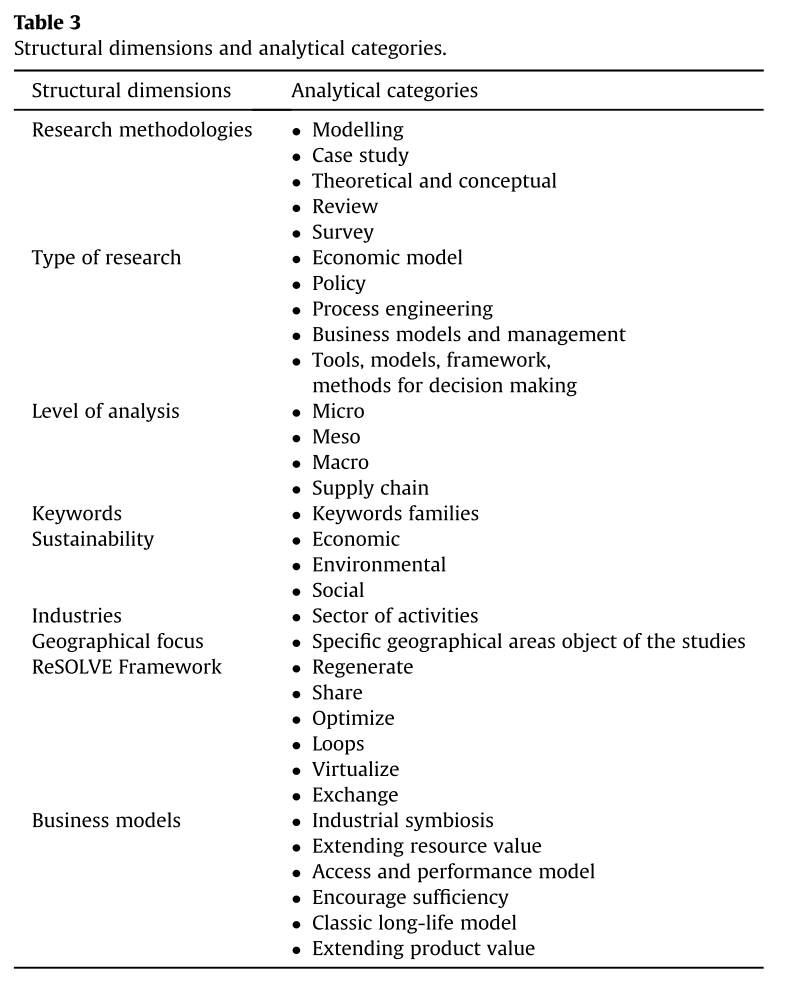
\includegraphics[width=0.8\textwidth]{sections/asset/cateogories of research.PNG}
    \caption{Cateogories of research}
    \label{fig:research cat}
\end{figure}


\subsection{Sustainability as contested}


\parencite{Stimson2006}


\begin{figure}[h!]
    \centering
    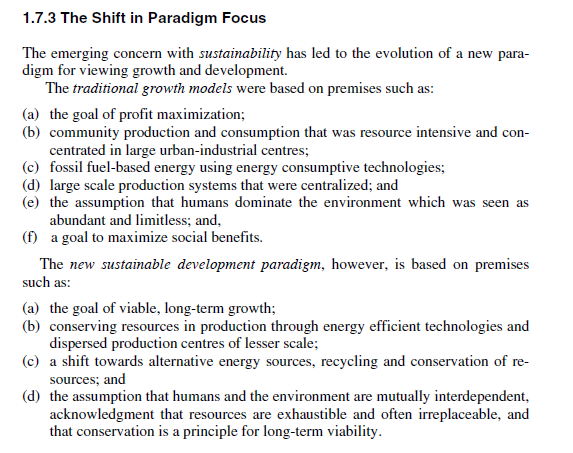
\includegraphics[width=0.8\textwidth]{sections/asset/shift.PNG}
    \caption{Change in paradigms}
    \label{fig:shift}
\end{figure}

Also on GIS

It is necessary to say something briefly about DSS in general. The goal of DSS is to focus ill-structured problems. As Densham (1994, p. 207) notes, DSSs are important when decision-makers “find it hard to define…problems and to articulate characteristics that they would like to see in a solution”. He argues that attributes of DSS include:\par
(a) support for the identification and use of data;\par
(b) the ability to represent complex relations among data which are needed for search, modelling and visualization;\par
(c) an architecture that is flexible enough to enable the user to combine model- ling and data in a variety of ways;\par
(d) an ability to generate a variety of types of output;\par
(e) a single, integrated, user interface which supports a variety of decision making styles; and\par
(f) an architecture that supports the addition of new capabilities as user needs evolve.




The new paradigm suggests that

This emerging new paradigm for regional economic development favours regions that have the human capital and technologies necessary to generate new knowledge and information—and to competently reinvent it—that creates the strategic architecture to facilitate a services dominated economy. The new paradigm will force regions to closely examine:
(a) what factors give them competitiveness? and \par
(b) how they may combine resources, competencies, assets, human capital and knowledge to become more efficient to create environments favourable for new economic development opportunities?\par
This paradigm assumes added significance when linked to another new paradigm being driven from an agenda that relates to ecological and resource capacity to support human populations and greater demands for economic equity. This is one of the great issues facing governments and communities throughout the world, including regional economies in the future. How we ensure economic development is more sustainable and equitable without forfeiting competitive advantage is uncertain and represents a significant challenge in formulating regional development strategies and for implementing plans.\par

During the 1990s, thinking on the new paradigm based on the concept of collaborative advantage (Huxham 1996) has advanced considerably, based on the prem- ise that networks, alliances, and partnerships are the replacing the more interventionalist strategies of the past, and these changes in strategic thinking (Hamel 1996; Mintzberg and Quinn 1992) are becoming more important and are being more fully incorporated in regional economic development strategy under con- temporary conditions of globalization, fast and flexible change. Strategy itself is also undergoing a major transformation, with a clearer separation of planning from strategy (Mintzberg 1994). As discussed in Chap. 5, strategy is now more the framework that provides a path for development and a direction for planning; it precedes planning. Planning is now being seen more as the instruments providing the mechanism for strategy implementation. Future regional economic development strategy will likely have three important functions. These are to:
(a) Identify key elements of capacity building to support economic development– the key elements of capacity building are what termed the strategic architecture of a region. \par
(b) Define strategic intent, in terms of the direction, destiny and discovery of opportunities for economic development in a region. \par
(c) Define the main thrusts of strategies for achieving strategic intent for managing economic development processes and for capacity building in a region—setting a future path. \par
The role of planning is to provide the details of initiatives, actions, resources, management, timing and delivery of resources, infrastructure, competencies and other supporting structures to execute strategy. Strategy is thus continuous and dynamic, while planning is more methodical and applied to the achievement of specific projects and outcomes.


The strategic architecture Hamel and Prahalad (1994) - \par
Much of the strategic architecture that can support the economic development of regions in the future similarly will be invisible or intangible. In the past, the strategic architecture of regional economies where their development was driven by comparative advantage, were strong in physical, financial and geographic terms. However, the strategic architecture required for regions to be successful in the ‘new’ economy of the contemporary global era is more in the form of technology, knowledge base and the virtual. Much greater knowledge is required about how to create that strategic architecture. This is where new tools for strategic planning—like multi-sectoral analysis (MSA) discussed in Chap. 7—can play a useful role in helping to develop strategic architecture by identifying:\par
(a) what competencies a region needs to build or maintain;\par
(b) what sector markets a region needs to develop or maintain;\par
(c) what strategic infrastructure to develop; \par
(d) what endowed resources to conserve and manage; and \par
(e) what approach to take to developing marketing intelligence.\par

The Challenge of the Virtual Economy
The development of communication technologies which enable organizations, institutions, and individuals to operate and manage activities in virtual space and communicate in virtual reality is changing significantly the conduct of business, social and economic transactions. The impact of the virtual economy may not be as profound as some writers would have us believe. It will, however, likely necessitate rewriting the rulebook of economic development practice. The virtual economy is the product of the information age. It is difficult to describe or define, but it is multi-dimensional and many of its elements are digital. There are many components of the virtual economy. These include:\par
(a) Organizations acting as brokers or catalysts for out-sourcing, coordinating, exchanging or disseminating goods and services using mainly telecommunications.\par
(b) The use of networks and alliances for business and other purposes. (c) Virtual simulation of events or experiences for recreational, commercial or re- search purposes and face to face video conferencing between people for consultation, inquiry, education and learning.\par
Almost every part of society in the developed world is being touched by the virtual economy and increasingly will be in the near future, as will also become the case in the developing regions.\par


\subsection{Urban and regional Planning}
\parencite{Friedmann1993}
'But what we are living through in the final decades of this century (1993) is something altogether different. It is nothing less than the collapse of the Euclidean world order of stable entities and common sense assumptions that have governed our understanding of the world for the past two hundred years.'
'We are moving into a non-Euclidean world of many space-time geographies, and it is the recognition of this change that obliges us to think of new and more appropriate models.'\par

[DEFINITION OF PLANNING]:
Planning is that professional practice that specifically seeks to connect forms of knowledge with forms of action in the public domain.'\par

'(...) we need first to consider the implications of the contemporary collapse of the time-space continuum. What would be the appropriate time and space of a non-Euclidean form of planning? The time of such planning is the \textit{real time} of everyday events rather than imagined future time.'\par

'Viewed in this light, planning becomes less a way of preparing documents, such as analyses and plans, and more a way of bridging planning knowledge and practice to bear directly on the action itself.'\par

'Concern with an imagined future will continue to play an important role in planning, but the emphasis in non-Euclidean planning should be on processes operating in actual or real time, because it is only in the evanescent and still undecided present that planners can hope to be effective.'\par

'As for the space of planning, we need to privilege \textit{regional and local} over national and transnational planning. This leads to a decentered view of planning 
-> 1. Heterogeneity of local places \par
-> 2. Organized civil society \par
-> 3. Regions and localities are the spaces of people's everyday lives. National and transnational space is typically for corporate actions and super ordinate bureaucracies.\par






\parencite{Casella2007}
'I have no quarrel with Friedmann’s characterization
of the non-Euclidian planning model as normative, innovative, political, transactive, and based on social learning. Those characteristics are validated by my own experience. But, I would add four other characteristics to Friedmann’s five, and call it a quantum model. A quantum planning model would also be technological, multidisciplinary, substantive, and intellectually free:'
description...



\parencite{WongTai-Chee;YuenBelinda;Goldblum2008}


Indeed, the concern with sustainable urban development arises and takes place in a world of economic globalization and of technological revolution, a world where the financial market’s selective expansion and innovation in the realm of communications systems has benefited strategic urban locations specifically catalytic to economic growth. Cities having built up a silent but revolutionary capacity in mastering flows (goods, people and information), in terms of paths and speed could affect their position and functions, their scale and ability in coping with these issues. If the rise of ecological ideas and consciousness in the early 1970s has been associated with “zero economic growth” (a concept promoted by the Club of Rome during the first oil crisis) and with the ideals of small/local dimensions (Schumacher 1973), the relationship between global dynamics and local development as expressed by the notion of “glocalism” are associated with mega-urban dimensions. The processes leading to this new representation of urban growth, the way to master its effects at urban, territorial and world scales, and to match it with the ideal of “sustainable development” naturally question the significance and the very nature of urban planning.\par

The objective of spatial planning for sustainability is primarily to counter the adverse effects of urban developments by means of systematic and organized land use planning activities. Sustainability planning has a holistic outlook which calls for an integration of the goals of the three Es (Economic, Environmental and Equity concerns) into an organized coherent system for a long-term objective formulation and plan implementation. No country can or should conduct sustainability planning in isolation, as the “stretching and deepening of global-scale processes” has exerted intricate interaction and reaction in one way or another on local scales (see Olds 2001: 19).\par



In terms of objectives, planning was no more dedicated to solving urban problems (in the sense of a corrective urbanism), but as a way to rationalize the city machinery itself, and to make it an efficient engine for nation-building and economic development.  










\subsection{Circular Economy}


About the concept \parencite{Prieto-Sandoval2018}



\parencite{Yuan2006}

\begin{figure}[h!]
    \centering
    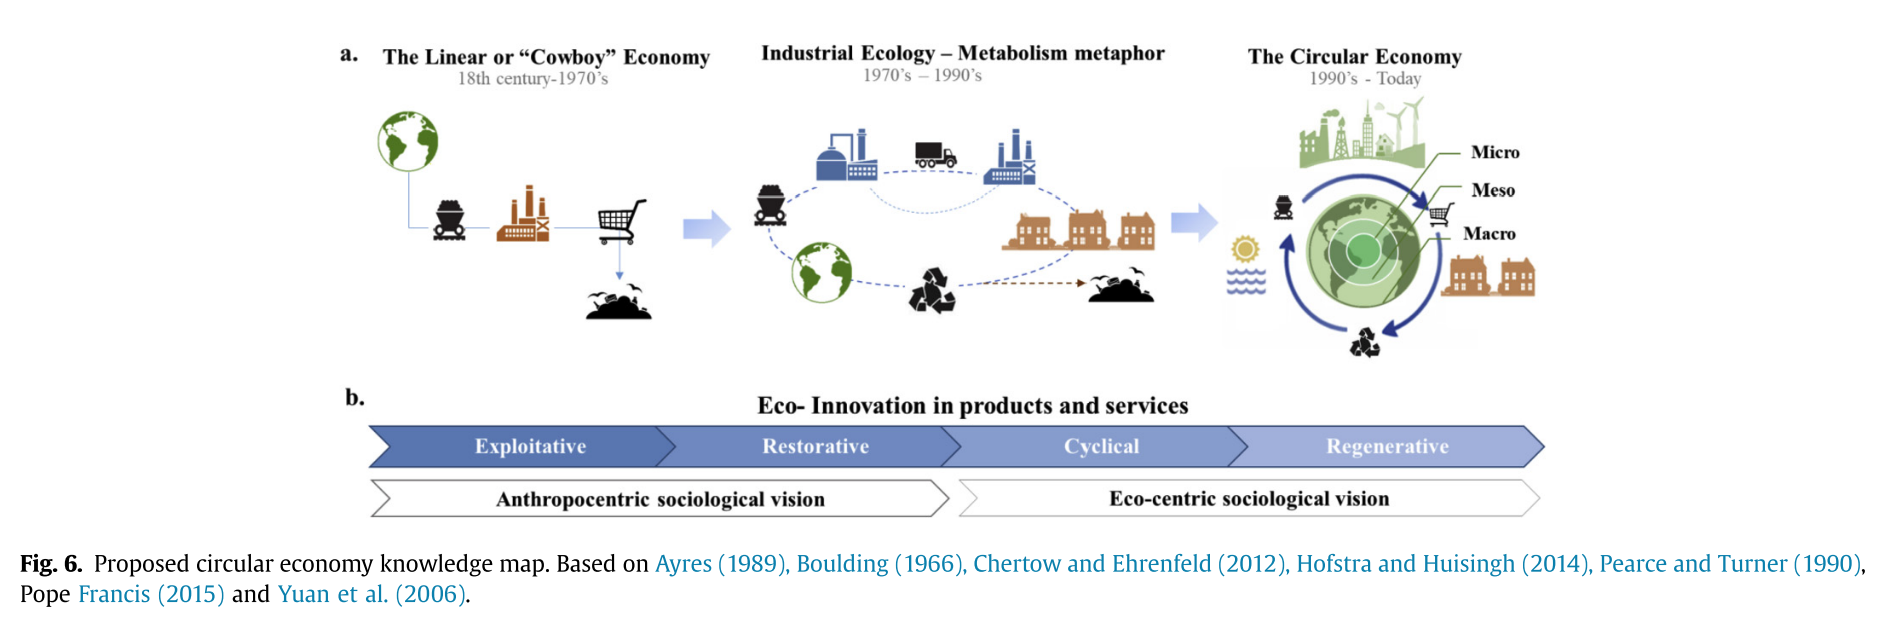
\includegraphics[width=0.8\textwidth]{sections/asset/model_strips.PNG}
    \caption{Models of economy}
    \label{fig:econ_models}
\end{figure}



\parencite{Gregson2015}
The concept of the circular economy has gained increasing prominence in academic, practitioner and policy circles and is linked to greening economies and sustainable development. However, the idea is more often celebrated than critically interrogated. Analysis shows the concept circulates as an idea and ideal, exemplified by industrial symbiosis and extended product life. Yet, its actual enactment is limited and fragile. Instead, circular economies are achieved mostly through global recycling networks which are the primary means by which wastes are recovered as resources. European policies eschew these circuits. Resource recovery through global recycling networks is regarded as a dirty and illegal trade. In its place, EU circular economies attempt to transform wastes into resources within the boundaries of the EU. Through an analysis of two case studies of resource recovery in the United Kingdom, we highlight the challenges that confront making circular economies within the EU, showing that these are borne of a conjuncture of politically created markets, material properties and morally defined materials circuits. We show resource recovery in the EU to be framed by moral economies, driven by discourses of ecological modernization environmental justice and resource (in)security, the last of which connects to China’s resource-intensive development.

This paper has subjected the concept of the circular economy to critical interrogation, by examining its instantiation in real world economies. The concept is an endlessly recited ideal. Yet, to effect a circular economy driven by producers through either industrial symbiosis or cradle-to-cradle manufacturing would require radical transformations to the economic order, including fundamental recasting of manufacture, retail, consumption and property rights. Beyond the ideal, in the messy world of how circularity is being enacted in actual economies, post-consumer wastes have become the basis for circular economies. One way in which this occurs is through global recycling networks, and new research has done much to make these activities visible. However, they do not count as appropriate forms of resource recovery and recycling in EU policies, where they are regarded as deeply suspect. Instead, under the rubric ‘high-quality recycling’, policy aims for the transformation of waste to resource within the EU. \par 


The question that remains is what form of politics lies behind this increasingly moral European market in resource recovery. There are three answers to this question. The first is a technocratic politics.
One element to this rests in the EU’s condemning of landfill.The underlying premise of this technocratic politics, however, is the technical dream of the perfect circle achieved via perfect recovery. This is technologic- ally impossible, as is illustrated by both dry recyclables and anaerobic digestion, both of which, whilst they recycle, also generate troublesome wastes as remainders of processing, and which continue to rely on landfill and/or incineration for their disposal. The second form of politics is environmental, driven by environmental
justice concerns. In continuing to portray global recycling as the global dumping of wastes on the people and environments of the Global South by the consumers and businesses of the Global North, accounts imply that global circuits of materials break the circular economy.

The third form of politics framing the morality of the EU’s circular economies is located in the political economy of resources and particularly resource security. For the most part, this politics is articulated in terms of the degree to which EU resource demand can be met through secondary resources. Answers range from around 50 per cent with respect to certain materials, such as paper and iron and steel, but much less for many others, even with a technically impossible 100 per cent recovery rate, and there are some 14 raw materials, mostly metals, which feature on the ‘high’ supply risk list for the EU economies. These are metals critical to high-value EU-based manufacturing, including in the aerospace, automotive and communications sectors. The figure that haunts these discussions though is China, and its resource-intensive form of development, particularly fears that it is securing control of resources from Africa. Indeed, the vulnerability of important sectors of EU manufacturing to Chinese resource use has been demonstrated recently through China’s dramatic cut-backs in rare earth metal exports. With China accounting for 95 per cent of global rare earth supply, the 30 per cent export reduction of 2010 led to rapid price hikes and a much-publicized rare earth panic in the United States, EU and Japan.






The concept and research is at an infant stage and the lack of a proper operational definition makes it and Essentially Contested Concept \parencite{Korhonen2018}. 

'However, the CE approach has almost exclusively been developed and led by practitioners, i.e., policy-makers and business development agencies such as business consultants, business associations, business foundations etc. (e.g., EMAF, 2013; COM, 2014; CIRAIG, 2015). From a scholarly position, the conceptual discussions on CE are still in their infancy and the literature is only emerging.'

After the review, a proposal of the definition is made.

'CE is a sustainable development initiative with the objective of reducing the societal production-consumption systems' linear material and energy throughput flows by applying materials cycles, renewable and cascade-type energy flows to the linear system. CE promotes high value material cycles alongside more traditional recycling and develops systems approaches to the cooperation of producers, consumers and other societal actors in sustainable development work.' 


Circular Economy is not yet a new paradigm, mainly because is still not embedded in every day life. 

As a consequence of identifying CE as a cluster concept it is vital that future research is careful with the framing of its studies. We have, in particular, identified the unit of analysis as a critical aspect of capturing CE research, since CE can have a very wide span both in terms of research topics and the scope of the study 

We propose a model for categorization that supports CE researchers in differentiating between different research streams and foci (see Fig. 2). Through better framing of the research it will also be easier to evaluate the quality of the research

\parencite{CDR2005}


\begin{figure}[h!]
    \centering
    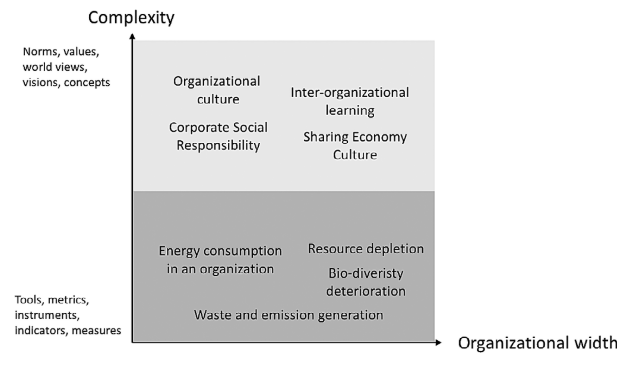
\includegraphics[width=0.8\textwidth]{sections/asset/stages_in_ce.PNG}
    \caption{Conceptual framework for CE research}
    \label{fig:stages}
\end{figure}


Using the umbrella concept in \textcite{Blomsma2017} conclude that whereas the various resource strategies grouped under the CE’s banner are not new individually, the concept offers a new framing of these strategies by drawing attention to their capacity of prolonging resource use as well as to the relationship between these strategies. As such, the CE offers a new perspective on waste and resource management and provides a new cognitive unit and discursive space for debate. 
Hirsch and Levin (1999) define an umbrella concept as: “a broad concept or idea used loosely to encompass and account for a set of diverse phenomena” (Hirsch and Levin (1999), 200). Umbrella concepts create a relation between pre-existing concepts that were previously unrelated, or not related in the manner the umbrella concept proposes, by focusing the attention on a particular shared quality or characteristic of the concepts it encompasses.


\begin{figure}[h!]
    \centering
    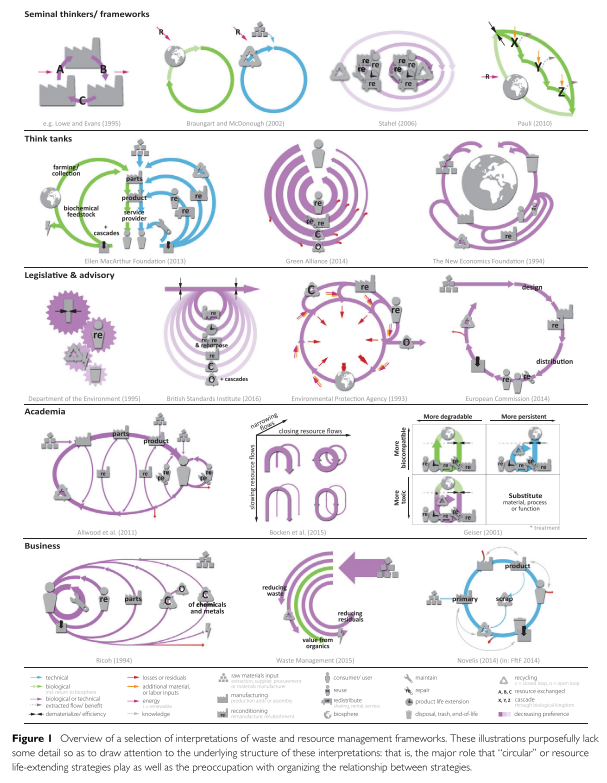
\includegraphics[width=0.8\textwidth]{sections/asset/ce_frameworks.PNG}
    \caption{Circular Economy frameworks}
    \label{fig:ce_frameworks}
\end{figure}

First, umbrella concepts typically arise when a field or discipline lacks guiding theories or a development paradigm.
Second, umbrella concepts typically progress along a predictable trajectory. This trajectory starts with the articulation of the umbrella concept by grouping pre-existing concepts. This phase is characterized by excitement and enthusiasm as the concept seemingly resolves the problem of too many unconnected concepts by providing a new framing that binds them together. After this phase, an umbrella concept usually sees its validity challenged when attempts at operationalizing the concept bring to the surface unresolved issues regarding its definition and assessment. A plurality of definitions, a lack of tools, and the existence of different indicators surface during this stage, raising questions regarding the nature of the binding capacity of the umbrella concept. This

\begin{figure}[h!]
    \centering
    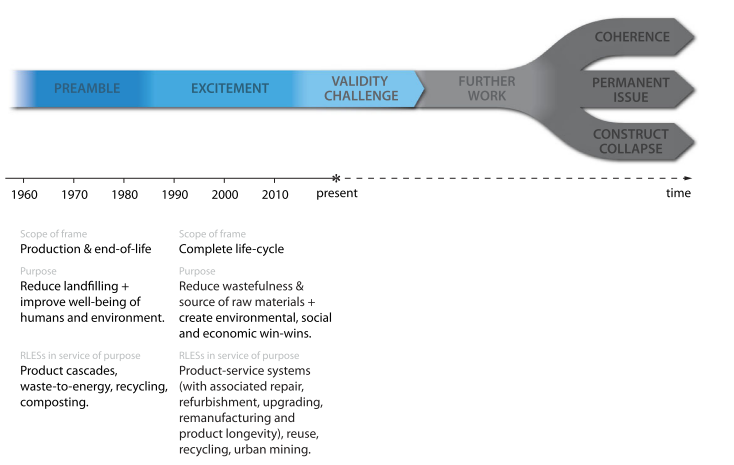
\includegraphics[width=0.8\textwidth]{sections/asset/ce_fork.PNG}
    \caption{Circular Economy trajectory}
    \label{fig:ce_trajectory}
\end{figure}


We are in the phase were the validity of the concept is being challenged. For instance, \parencite{Gregson2015,Gregson2015,Murray2017}, argue whether current interpretations are indeed in line with the creation of both societal and environmental benefits.

Not only quantitative work is needed. In order to make a socio-technical transformation other non-engineering questions need to be addressed. 

That is: Whereas answers to technical and engineering what questions are needed, which IE has traditionally engaged, what is also required if CE strategies are to be implemented are answers to how questions regarding accomplishing socioinstitutional change


\textcite{Korhonen2018a} However, the concept of CE and its practice have almost exclusively been developed and led by practitioners, i.e., policy-makers, businesses, business consultants, business associations, business foundations etc. (see e.g. EMAF, 2013; COM, 2014; CIRAIG, 2015). The scientific research content of CE remains largely unexplored. Ecological economics may be the most fruitful source from which the new practical, policy and business orientated concept of CE could find scientific and theoretical sup- port and guidance. Ecological economics has a long tradition in recycling and other CE-type concepts on the macroeconomic level al- though not presented under the CE term. Also on the microeconomic level, CE-type papers have been published in ecological economics



\textcite{Levoso2019} propose a methodology to implement CE in urban areas. This is based on the analysis of specific case studies on urban implementations.

\begin{figure}[h!]
    \centering
    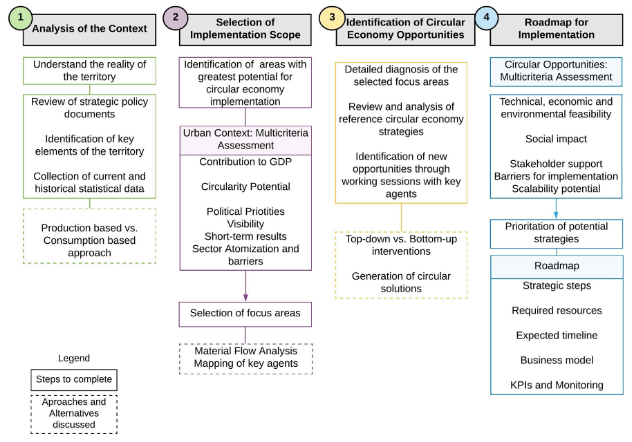
\includegraphics[width=0.8\textwidth]{sections/asset/ce_in_cities.PNG}
    \caption{Methodological proposition to apply CE in cities}
    \label{fig:ce_application}
\end{figure}


\parencite{Korhonen2018a}
Circular economy (CE) is a concept currently promoted by the EU, by several national governments including China, Japan, UK, France, Canada, The Netherlands, Sweden and Finland as well as by several businesses around the world. The European Commission recently esti- mated that circular economy-type economic transitions can create 600 billion euros annual economic gains for the EU manufacturing sector alone (COM, 2014; EMAF, 2013;see also CIRAIG, 2015 and COM, 2015). Finland's Independence Celebration Fund (FICF, SITRA) and Mckinsey (2014) jointly estimate 2.5 billion euros annual gains for the national economy of Finland through circular economy. The global economy would benefit 1000 billion US dollars annually (FICF and Mckinsey, 2014;see e.g. EMAF, 2013). China, as the first country in the world, adopted a law for the circular economy in 2008 (CIRAIG, 2015). Circular economy is recommended as an approach to economic growth that is in line with sustainable environmental and economic develop- ment (see EMAF et al., 2015; EMAF, 2013; EMAF, 2012; CIRAIG, 2015; COM, 2015; COM, 2014).


The scientific and research basis of the CE approach seems to be only in its infancy. To authors' knowledge the definition given above in section three (3) is the first attempt to present a scientific research-based definition of CE. Many key questions are still open. These will arise, e.g. from the nature of self-organized complex social-ecological systems (see e.g., Chertowand Ehrenfeld, 2012; Folke, 2006) to which CE systems belong.


\begin{figure}[h!]
    \centering
    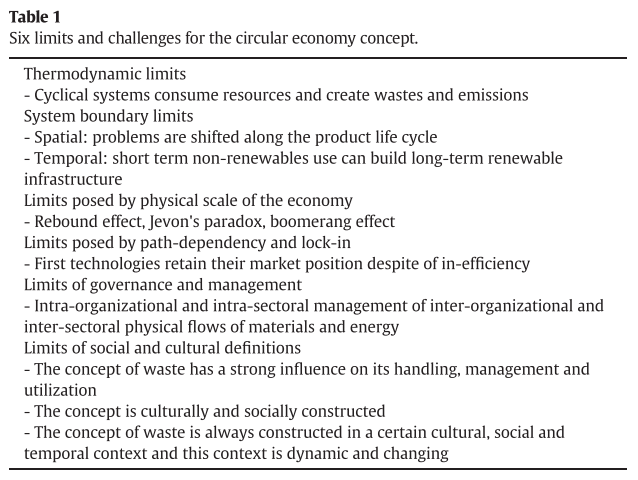
\includegraphics[width=0.8\textwidth]{sections/asset/limits.PNG}
    \caption{Six limits of the concept of CE}
    \label{fig:ce_limits}
\end{figure}


\parencite{Stahel2013}


To overcome this general lack of knowledge, Stahel (2013) outlines a set of principles that would apply in a Circular Economy: (a) the smaller the resource circulation (activity-wise and geographically) the more profitable and resource efficient; (b) material loops are continuous, therefore, materials constantly circulate in the economy and feed into new production processes, minimising potential waste; (c) maintaining the value, quality and performance of goods; (d) the efficiency of managing stocks in CE increases with a decreasing flow speed; (e) extending ownership is a cost-efficient strategy, as reuse, repair and remanufacturing without ownership changes saves on transaction costs; and (f) CE requires the existence of well-functioning second hand product and secondary materials markets. Skene (2017) presents a similar set of principles, and complements further with (g) elimination of toxic substances and (h) renewable energy use.



\parencite{Milios2018}
From a sustainability point of view, CE has been found to lack on considerations towards the social dimension (Broto et al. 2012; Jiao and Boons 2014; Murray et al. 2017). However, Murray et al. (2017) identified that some elements of relevance do exist in the CE narrative, referring to the maximisation of ecosystem functioning and human well-being, apart from the obvious tenet of job creation (locally). Moreover, the strong ‘‘material’’ focus in the current narrative of CE seems to preclude wider systemic considerations of sectoral approaches to CE (Haupt et al. 2017). 

\begin{figure}[h!]
    \centering
    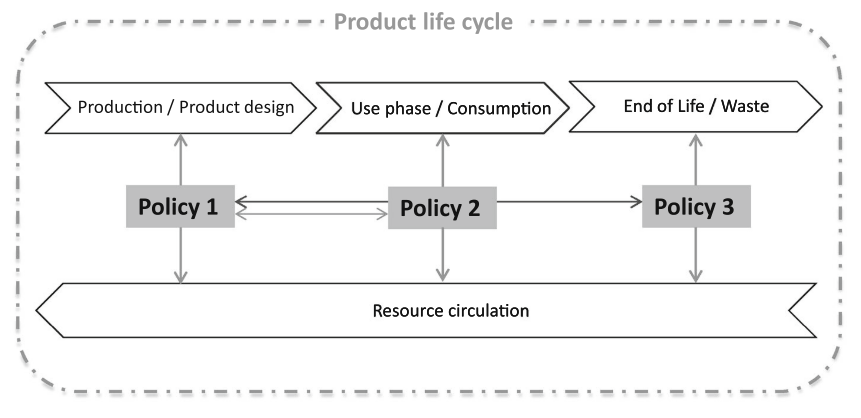
\includegraphics[width=0.8\textwidth]{sections/asset/policies.PNG}
    \caption{Product life cycle and policies}
    \label{fig:ce_policies}
\end{figure}


Nicolli et al. (2012) point out that there is a significant risk of high search and transaction costs associated with recyclable materials in secondary markets, related to incomplete information. There is usually a lack of information concerning the quality and properties of potentially recyclable or reusable materials and products. In addition to this, the provided information is usually asymmetric, in the sense that the supplier holds a negotiating advantage by knowing more about the quality or properties of the material or product than the potential buyer. In such cases, a broad range of policy instruments can be used to support the markets. The establishment of harmonised quality standards for recycled materials and/or certification schemes could be useful in overcoming such barriers (Finnveden et al. 2013)



about measuring Indicators
\parencite{Geng2012}

\begin{figure}[h!]
    \centering
    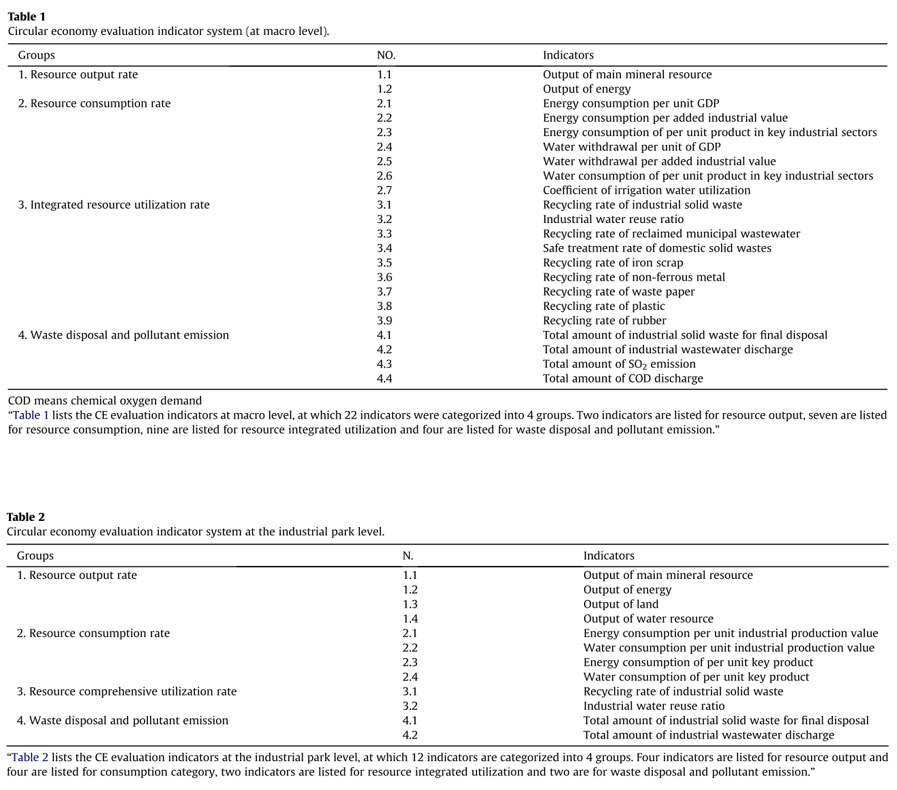
\includegraphics[width=0.8\textwidth]{sections/asset/ce_china_indicators.PNG}
    \caption{Circular Economy indicators in China}
    \label{fig:ce_chinaindi}
\end{figure}



\parencite{eliaMeasuringCircularEconomy2017}
critical of chines indicators


\subsection{Barriers to Circular Economy}


\parencite{Kirchherr2018}

We present the first large-N-study on circular economy barriers in the EU (208 survey respondents, 47 expert interviews). We find that cultural barriers, particularly a lack of consumer interest and awareness as well as a hesitant company culture, are considered the main circular economy barriers by businesses and policy-makers. These are driven by market barriers which, in turn, are induced by a lack of synergistic governmental interventions to accelerate the transition towards a circular economy. Meanwhile, not a single technological barrier is ranked among the most pressing circular economy barriers, according to our research. Overall, our work suggests that circular economy is a niche discussion among sustainable development professionals at this stage. Significant efforts need to be undertaken for the concept to maintain its momentum. \par

\begin{figure}[h!]
    \centering
    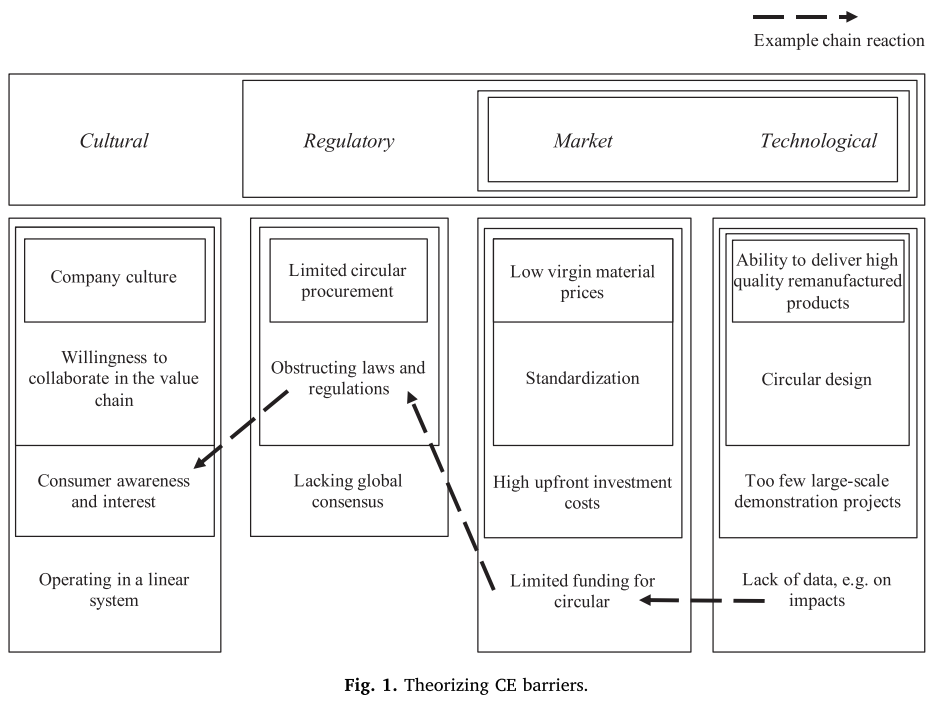
\includegraphics[width=0.8\textwidth]{sections/asset/barriers.PNG}
    \caption{Barriers to implement CE}
    \label{fig:ce_BARRIERS}
\end{figure}

\begin{figure}[h!]
    \centering
    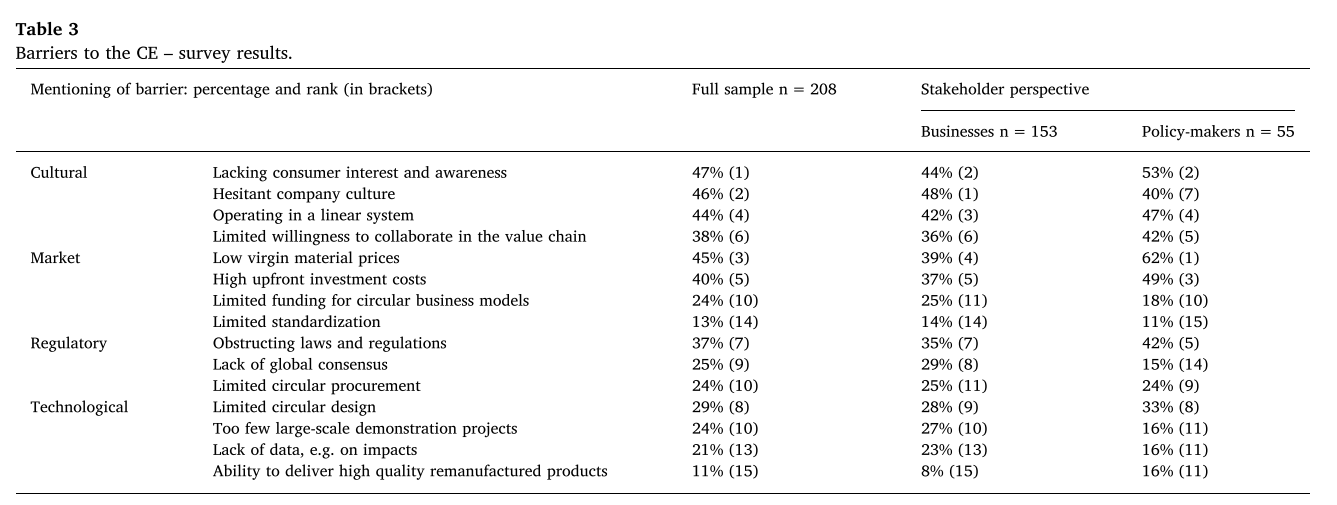
\includegraphics[width=0.8\textwidth]{sections/asset/BARRIER_SPECS.PNG}
    \caption{Survey results}
    \label{fig:ce_BARRIERS}
\end{figure}

The CE concept is gaining momentum these days as an allegedly
novel pathway towards sustainable development. Particularly the EU has endorsed the concept. Despite the growing attention and endorsement received, the CE has seen limited implementation so far. Those writing on the CE frequently blame the limited CE implementation on various barriers, with technological barriers having emerged in the literature as the alleged core barriers that impede the transition towards a CE. \par


\parencite{Shahbazi2016}
\begin{figure}[h!]
    \centering
    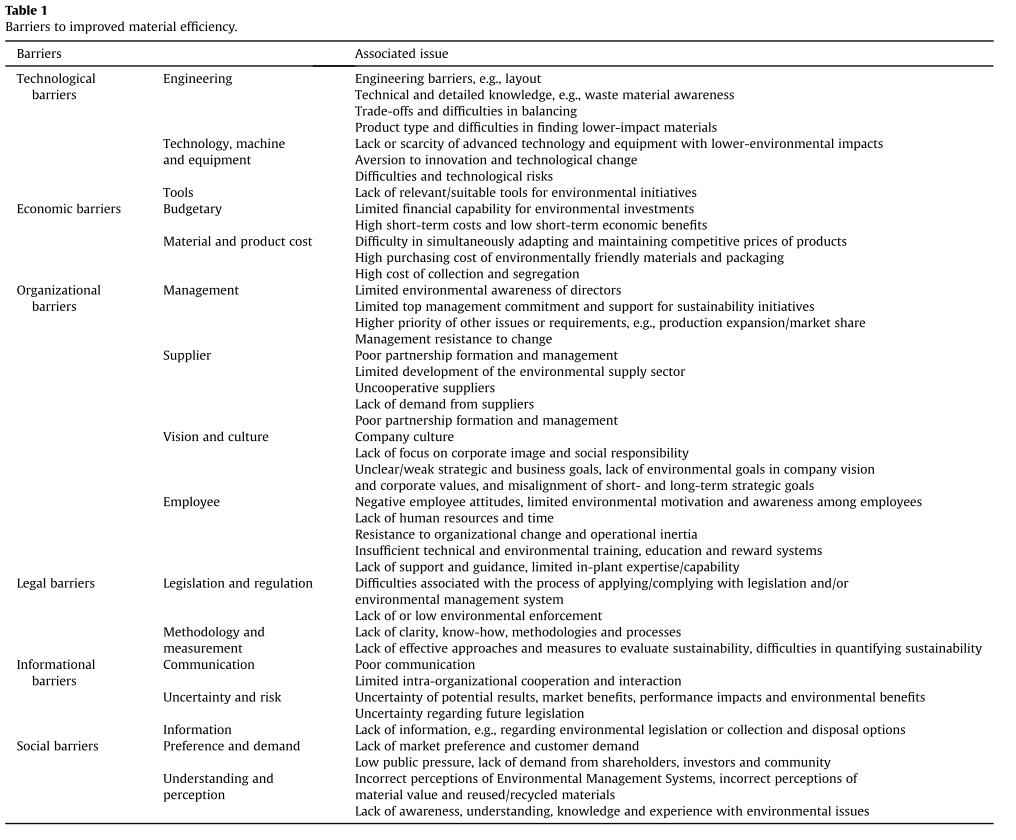
\includegraphics[width=0.8\textwidth]{sections/asset/more_barriers.PNG}
    \caption{More barriers to improve resource efficiency}
    \label{fig:ce_BARRIERS1}
\end{figure}


\parencite{Ritzen2017}
These barriers relate to what CE is – barriers for closing material loops, delivering new offers to customers, making requirements and expectations of suppliers and on customers, and developing the whole supply chain. Also, how their current businesses are conducted is strongly connected to these barriers. When analyzing the case companies in greater detail, we also see barriers rather related to the actual transition towards CE, and they tend clearly to concern integration of different perspectives and of different domains. These barriers are in several ways similar to barriers to integration of environmental aspects, though is likely challenges of larger altitudes as they encompass every function and every level in the organization and take sustainability issues to a strategic level. These working way that is needed for performing the required disruptive changes and radical innovations. \par


Finally, as an integration barrier we see the lack of
integration throughout the supply chain, also identified among respondents. Possible solutions for closing material loops are requiring a closer connection between suppliers and producers and between producer and customers. The characteristics of these two different companies matter for which barriers are revealed, in relation to their business logic.However, what they have in common is that also for disruptive changes more collaboration is necessary for innovation in the eco-systems of different actors [37, 38]\par

In addition to integration barriers, the barrier connected to knowledge and an exploratory way of working needs to be addressed.
Knowledge is not only of concern for its content, with lack of knowledge as a barrier, but also for how companies regard knowledge creation and how this is managed within innovation. The ability to perform radical innovations is strongly connected to an explorative way of working, deeply connected to how knowledge is gained. In exploration, knowledge is looked for outside the company, and experiments are made for learning purposes in invention activities [24].\par


\parencite{Ritzen2017}

\subsubsection{Overcoming challenges}
\parencite{Bressanelli2018}

\parencite{Okorie}

\subsection{Circular Flow of resources}








\subsubsection{Industrial Symbiosis}



\parencite{Almeida2015}
strategies for cleaner production
\begin{figure}[h!]
    \centering
    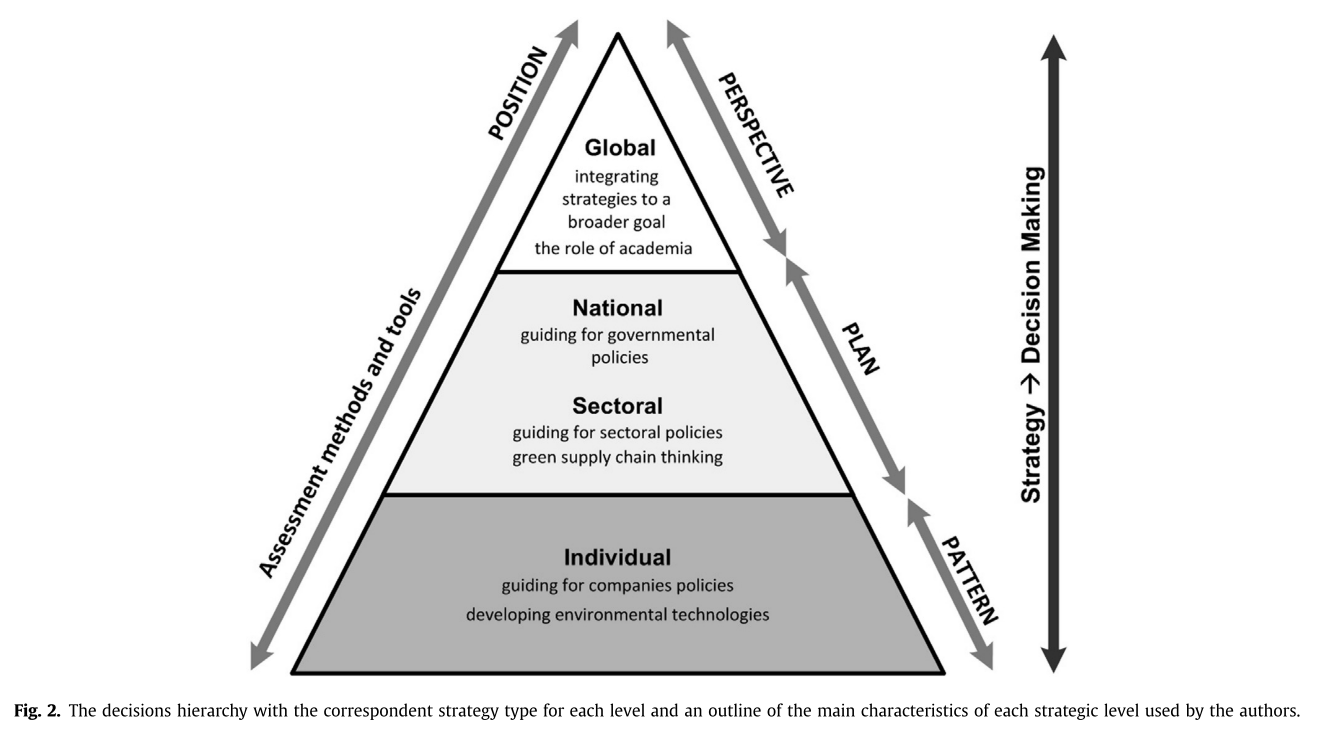
\includegraphics[width=0.8\textwidth]{sections/asset/clean production.PNG}
    \caption{Clean production strategies}
    \label{fig:cp_stategies}
\end{figure}

{Industry 4.0}



\subsubsection{Waste}
\parencite{OakdeneHollins2017} - Towards a circular economy - waste mgmt in the eu

{Industry 4.0}
\parencite{Vafeiadis2019}









%\section{Concepts}


\subsection{Glossary}

\textbf{Symbiosis: }

Circular Economy

Sharing Economy

Industrial Synergy

Agent-Based Model

Complex System

Internet of Things


Industrial Ecology
Material Flow Analysis


Sustainable Development Goals


United Nations


Industrial Symbiosis Dynamics

Cleaner production


Product-service systems (PSS) are

Bounded rationality

Embeddedness

Eco-Industrial Parks

Life cycle assestment

Material flow analysis
circular business models (CBMs) 

Resilience

Sustainability

by-product synergy (BPS)

Local Authorities

Public Private Partnership PPP

Place promotion or ‘boosterism’ (Short, 1999; Prytherch, 2002)


Closed loop 

Sustainable development

Local Agenda 21

Zero Waste Manufacturing 

Emergy is a measure of real wealth, defined as “the sum of available energy of one kind previously required directly and indirectly through input pathways to make a product or service”

3Rs (recycle, reduce and reuse)
Resource recovery (RR)
In-house reuse

Cost-Benefit analysis

Institutional capacity

Industrial poles

Industrial Symbiosis Network
Resilence

sustainable production and consumption (SPC)
triple-bottom-line (TBL) decision-making
institutional capacity building.

By-product synergy (BPS) : It consists in the maximization of resources utilization with the replacement of raw materials by by-products as inputs for industrial processes. In

Sustainability-Oriented Cooperation

\subsection{Methods}
MIND Method -> Method for analysis of INDus-
trial energy systems [18,19]. It is based on mixed integer linear programming (MILP) and has mainly been used for modelling industrial plants and to some extent for modelling the interac- tion between an industry and a district heating system [20,21].
(Karlsson2008)

\subsection{Case studies}
\textbf{Tampico, Mexico}
Midong Chemical Industrial Park (MCIP), China
Kalundborg, Denmark
Viotia region, Greece
Kawasaki’s experience JPN IRON/STEEL

Jinan and Liuzhou of China
Liuzhou city
Liuzhou and Jinan Liang, China - IRON/STEEL
Handelo bioenergy complex, Norrkoping, Sweden
Barceloneta, Puerto Rico. 
recycling network Styria in Austria, 
recycling network Oldenburger Munsterland in Germany
manufacturing sector in Austria

Port of Cape Charles Sustainable Technology Park, USA
Devens Planned Community, USA
Londonderry Ecological Industrial Park, USA
Avtex Redevelopment Site, USA

Santa Croce sull’Arno

Tianjin Binhai New Area, China -> TEDA


Shandong Lubei eco-industrial park, china


\subsection{programmes}
\textbf{The Business Council for Sustainable Development, United Kingdom
national IS programme (NISP)}

Korean eco-industrial park scheme

Landskrona industrial symbiosis programme

Jiayuguan city is located in the western of China, which is a modern city that developed on the basis of Jiuquan Iron \& Steel Co., Ltd. (JISCO)

e-Symbiosis, Greece






\section{Research Aim and Objectives}































\subsection{General}
\textbf{\citetitle{Chertow2012}}\par
\textcite{Chertow2012} presents a discontinuous three-stage model used to describe the genesis of the process. While there is much variation, with no single path to this outcome, the recognition of benefits is seen as an emergent property characteristic of these self-organized systems that move beyond the initial stage. \par
-> Examples of 10 well-documented case studies \par
-> We do not yet have enough knowledge about industrial ecosystems to understand fully their life cycles and the categories into which they fall. Yet, what we are proposing moves beyond the biological notion of mutually beneficial exchange by two organisms toward network configurations involving many more. Specifically, the model they present applies to these 10 well-studied examples.


\begin{figure}[h!]
    \centering
    \includegraphics[width=0.85\textwidth]{Assets/Kalundborg.PNG}
    \caption{Evolution of industrial symbiosis of the Kalunborg region}
    \label{fig:Kalundborg}
\end{figure}


\textbf{\citetitle{Chertow2012}}\par
\textcite{Keckler1998} Linear and other mathematical programming approaches were used to evaluate water reuse opportunities. It is claimed that the methods used in this paper can be used to evaluate the potential reuse of other materials. \par
-> Case study of Bayport Facility:

\begin{figure}[h!]
    \centering
    \includegraphics[width=0.4\textwidth]{Assets/Bayport.PNG}
    \caption{Interaction of 3 manufacturers (M,O \& P) and 3 treatment steps (A, B \& C)}
    \label{fig:Bayport}
\end{figure}


\subsection{Industry 4.0}
\textbf{\citetitle{Kerdlap2019}}\par
\textcite{Kerdlap2019}, Zero Waste Manufacturing (ZWM) as a concept to help countries to support transition towards Circular Economy (CE). \par
The main focus is to eliminate waste across the entire supply chains.\par


\textbf{CASE STUDY:} Singapore\par
\textbf{CONTEXT:} Singapore lacks of land area to develop specific equipment which produces high prices. There is also a challenge of productivity and labor shortage.\par
\textbf{METHOD:} To identify the technologies that stakeholders can implement to achieve ZWM, this study proposes a holistic framework comprising six technology themes that aim to mitigate waste generation across the life cycle stages of production and consumption systems. These six themes include:\par

\begin{enumerate}
    \item design for zero waste
    \item smart waste audit and reduction planning
    \item smart waste collection
    \item high-value mixed waste processing
    \item collaborative platform for industrial symbiosis
    \item waste to resource conversion and recycling
\end{enumerate}\par

The authors identified the following benefits for each of the themes.
\begin{figure}[h!]
    \centering
    \includegraphics[width=0.8\textwidth]{Assets/s3.PNG}
    \caption{Stakeholders benefits under each theme of ZWM}
    \label{fig:ZWM}
\end{figure}

\textbf{RESULTS:} Main challenge for I.S. is to get a critical mass and be known\par

\textit{"Collaborative platforms for industrial symbiosis face few technical
barriers for implementation in Singapore. This technology relies primarily on digital systems and would require minimal to nearly no changes in physical infrastructure to implement (Yeo et al., 2019). Many sharing economy-based services are already actively used in Singapore and so a similar digital platform focused on waste to resource matching and exchanges between individuals and companies is technically feasible. One of the challenges that may arise during the initial stages of implementation would be achieving a critical mass of users for the collaborative platform to successfully facilitate industrial symbiosis exchanges. The impact on Singapore’s waste management system through implementing collaborative platforms for industrial symbiosis would be a reduction in the amount of waste materials that get mixed in with waste sent to incinerators. Instead, users would be directly matched to a market where their waste could be recycled to gain value and not need to rely on the existing waste collection and recycling system."} \par

Future research areas  6 identified:
\begin{enumerate}
    \item Smart bins that measure waste material composition:  
    \item Small and medium sized waste sorting technologies: 
    \item Matching consumers with remanufacturing services:  
    \item Life cycle impact evaluation models for IS platforms:
    \item Small scale food waste digesters: Dense urban settings present space limitations for implementing large scale digesters for recycling a region’s food waste. Implementation experience has shown that large scale digesters in urban settings face financial issues due to logistical challenges. Research is therefore needed in developing smaller food waste digestion systems that can be sited close to the source of generation such as residential areas or commercial dining areas and sized for the specific daily food waste volumes. The technical issues that need to be overcome are reducing odor and noise from the small scale digesters to avoid disturbance to people nearby 
    \item Reducing contamination of consumer waste streams: 
\end{enumerate}\par


\textbf{\citetitle{Tseng2018}}\par
\textcite{Tseng2018}, 

\textit{Moreover, gaps remain in operational data-driven and 3Rs optimization solutions, which may be the key components of industrial symbiosis practices.}
\textit{To close these gaps, corporate operational data must be disclosed within supply chain networks, and data-driven and optimization solutions for an industrial symbiosis network should be further addressed. In highly integrated systems with high levels of cyclic linkages, the shortcomings of data-driven and optimization solutions will amplify a magnitude of disruptions in the industrial symbiosis practice. The segment of the scientific community represented by Resources, Conservation and Recycling should leverage the technological innovations in Industry 4.0, using tools such as big data and IoT, to achieve gains across TBL perspectives.}
\textit{Regarding the gap in the literature, a search of the Scopus database using the keyword phrase “Data-driven on industrial symbiosis” yielded only 20 articles, few of which were related to industrial symbiosis. Thus, there is clear bibliometric evidence of the sparsity of scientific literature on this important topic. This gap presents an urgent challenge to the scientific community of industrial ecology as well as the scientific community of Resource, Conservation and Recycling to contribute concepts and tools to assist data-driven and optimization solutions in industrial symbiosis studies.}


\textbf{\citetitle{Ferrera2017}}\par
\textcite{Ferrera2017}

Presents a EU-funded collaborative project: MAESTRI. The MAESTRI Total Efficiency Framework (MTEF) aims to advance the sustainability of manufacturing and process industries by providing a management system in the form of a flexible and scalable platform and methodology based on four pillars: (a) an effective management system targeted at process continuous improvement; (b) Efficiency assessment tools to support improvements, optimisation strategies and decision support; (c) Industrial Symbiosis paradigm to gain value from waste and energy exchange; (d) an Internet-of-Things infrastructure to support easy integration and data exchange among shop-floor, business systems and tools.\par


\begin{figure}[h!]
    \centering
    \includegraphics[width=0.8\textwidth]{Assets/i1.PNG}
    \caption{Main gaps regarding the effective implementation of energy and resource management}
    \label{fig:mgmt_gaps}
\end{figure}



\textbf{\citetitle{Garcia-Muina2019}}\par
\textcite{Garcia-Muina2019}, aimed to test eco-design as a tool to define the equilibrium point between sustainability and circular economy in the manufacturing environment of ceramic tile production, and to demonstrate how new business opportunities can be created through evolution from a linear to a circular business model, thanks to IoT and Industry 4.0 technologies used as enabling factors. The main result of this paper was the empirical validation in a manufacturing environment of sustainability paradigms through eco-design tools and digital technologies, proposing the circular business model as an operational tool to promote the competitiveness of enterprises. \par
\textit{For manufacturing companies, the transition to circular business models (CBMs) can be hampered both by the lack of relevant data and by operational tools.}

\textbf{\citetitle{Hertwig2019}}\par
\textcite{Hertwig2019}
\textit{Industrial processes are changing because of the new challenges. Digitalization is a current topic which has huge influence on economical procedures. A main topic in this context is the German initiative “Industry 4.0”. New ways of thinking have a great impact on the way manufacturing is done and the digitalization opens up new possibilities. Current discussions on sustainability are influencing the economic thinking heavily. The importance of sustainable development with respect to environment and climate becomes more and more obvious to everybody (....) Nevertheless, society will only accept limitations, without a reduction of living quality. Based on that, it is necessary to implement a new procedures in existing structures. Additionally, it is required to implement changes without reducing economic potentials. The approach of symbiosis can support these developments. However, technology is a required extension to reach the target of sustainability. In}


\begin{figure}[h!]
    \centering
    \includegraphics[width=0.4\textwidth]{Assets/stut1.PNG}
    \caption{Levels of analysis for implementation of sustainability (with local interdependencies, in direct surrounding of company, within the company—increasing degree of detail)}
    \label{fig:indusrty_town}
\end{figure}


\textbf{\citetitle{Ares2019}}\par
\textcite{Ares2019}

Not relevant

\subsection{Big Data}
\textbf{\citetitle{Joshi2019}}\par
\textcite{Joshi2019}, deal with a thermal decomposition of plastics and tries to evaluate local opportunites of re-use of plastics. The papers builds and index of potenial places that can take advantage of their situation. \par
It works at country level, and I dont really like the way data in handled, it seems that there are some problems with correlation and dont really know how to use this index at a country level to produce local strategies. \par

\textbf{\citetitle{Davis2017}}\par
\textcite{Davis2017}, this paper takes a data science and novel approach to study sustainability. In this case, the authors uses NLP to understand the relationship between PRODUCT-WASTE of organic waste. \par
As an output an interactive tool is produced that can be used as an inspirational work. 

\begin{figure}[h!]
    \centering
    \includegraphics[width=0.4\textwidth]{Assets/NLP test.PNG}
    \caption{Web site created from these research. Below are the access links}
    \label{fig:nlp}
\end{figure}

\url{http://isdata-org.github.io/mapping-the-bioeconomy/TopicModelling/}
\url{http://isdata-org.github.io/mapping-the-bioeconomy/CoOccurrenceAnalysis/CircleCoOccurLayout.html}


\textbf{\citetitle{Migliore2020}}\par
\textcite{Migliore2020}, provide examples of waste treatment and a portfolio of

\textbf{\citetitle{Bin2015}}\par
\textcite{Bin2015}, some of the barriers for I.S. are explored. The paper proposes a general framework and suggests how Big Data could potentially be used in theory. In the paper, the usefulness and need to adopt new technological approaches is highlighted. 

\textit{This approach is proven by successful cases, but is constrained by land scarce cities as well as the limited types and scales of the companies that can be included in an industrial park. The paper proposes a big data analytics approach to realize industrial symbioses among the industries in a city's close proximity. The waste streams and resource requirements of existing companies are identified and matched with resources needs directly or indirectly through conversion processes. The viability, critical elements and technical challenges of the approach are discussed.}

\begin{figure}[h!]
    \centering
    \includegraphics[width=0.4\textwidth]{Assets/waste_paths.PNG}
    \caption{Tentative waste paths}
    \label{fig:waste_path}
\end{figure}

\begin{figure}[h!]
    \centering
    \includegraphics[width=0.4\textwidth]{Assets/data frame.PNG}
    \caption{Framework suggested}
    \label{fig:data}
\end{figure}

\begin{figure}[h!]
    \centering
    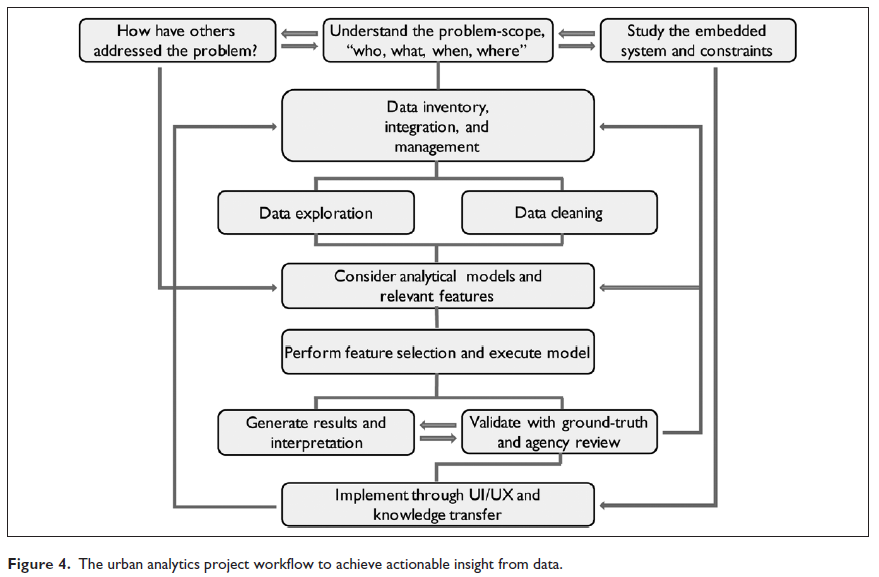
\includegraphics[width=0.4\textwidth]{Assets/data.PNG}
    \caption{Data and categorization of the model}
    \label{fig:datavars}
\end{figure}

\subsection{Networks}
\textbf{\citetitle{Chopra2014}}\par
\textcite{Chopra2014}, explore the dynamics of the Danish I.S. How did the symbiotic relationships evolved, what are the products or services exchanged. \par
Moreover, the aim of the study was also to deal with the resilience aspects of this I.S.
\textit{Since most of the industrial symbiotic networks are based on ad-hoc opportunities rather than strategic planning, gaining insight into disruptive scenarios is pivotal for understanding the balance of resilience and sustainability and developing heuristics for designing resilient IS networks. }
\textbf{CASE STUDY: } Kalundborg Industrial Symbiosis (KIS)

The present work focuses on understanding resilience as an emergent property of an IS network via a network-based approach. Scenarios are used to study resilience of the Case.

\textbf{\citetitle{Domenech2019}}\par
\textcite{Domenech2019}, \textit{The analysis is based on a combination of desk research, gathering of primary data from case studies, a survey to IS network facilitators (n=22) and in-depth interviews and focus groups (3) with IS practitioners, policy officers and industry representatives (n=25). The analysis identified pockets of IS activity across all Europe, although varying in nature, resources exchanged and scale and scope of the initiatives. The average size of the mapped networks is approx. 473 members, but the median is approx. 100 members, which indicates high variability of sizes. The geographical scope of the synergies also seems to be dependent upon the following factors: 1) the type of waste stream/by-product; 2) transport costs and 3) market value of secondary materials.}\par

\begin{figure}[h!]
    \centering
    \includegraphics[width=0.4\textwidth]{Assets/I.S. MAP.PNG}
    \caption{Map of case studies}
    \label{fig:casestudiesmap}
\end{figure}


\textit{The paper also discusses key obstacles facing IS development in Europe highlighting: 1) weakness of economic incentives given the low margin of IS projects associated to undeveloped secondary markets; 2) geographical variation of incentives and drivers, given differences in policy frameworks and support mechanisms (e.g. landfill tax levels) and 3) legislative issues that make transport over geographic boundaries extremely complex and administratively burdensome.}\par

The obstacles and determinants of I.S. are explored. The webpage of the project is down\par

From this paper a list of case studies and references can be extracted


\textbf{\citetitle{Ghali2019}}\par
\textcite{Ghali2019}, suggest that \textit{Industrial synergies join two or more organizations that initially functioned as independent economic actors that may originate from different sectors—together in order to share resources and exchange by-products for mutual environmental, financial, and social benefits for its participants. Industrial}.\par
\textit{In practice, the initiation of an industrial synergy, and particularly the identification of by-product compatibilities, relies on direct or facilitated knowledge and information sharing, which is essential for discovering industrial synergy opportunities.}\par
They propose a \textit{framework exploits the ability of the sematic web to enable the search for analogies between potential partners within a region or district and existing industrial synergies around the world.}\par
This requires (1) stakeholders to acknowledge their need to manage or acquire by-products, (2) data collection about waste and by-product flows and existing synergies, (3) potential synergy identification, and (4) some form of sharing data or contact between potential stakeholders.

\textbf{\citetitle{Morales2019}}\par
\textcite{Morales2019}, use the case study example of Altamira-Tampico in Mexico and study the I.S dynamics for a period of 20 years. \textit{The Industrial symbiosis emergence constitute a complex and dynamic process that we set in four different phases in this paper: Emergence, Regional efficiency, Regional learning, and Sustainable Industrial District.}\par
\textit{The industrial symbiosis at Altamira is depicted here as a centralized and ancillary industrial symbiosis embedding a socio-technical and environmental model, one of the most complete biophysical, social, and economic symbiotic case studies in Latin America.}\par



\begin{figure}[h!]
    \centering
    \includegraphics[width=0.4\textwidth]{Assets/Altamira.PNG}
    \caption{Map of Altamira-Tampico}
    \label{fig:altamiramap}
\end{figure}



\begin{figure}[h!]
    \centering
    \includegraphics[width=0.4\textwidth]{Assets/altamira dynamics.PNG}
    \caption{Typology of dynamics in Altamira}
    \label{fig:altamira_example}
\end{figure}




\textbf{\citetitle{Huang2019}}\par
\textcite{Huang2019}, produce a bibliometric analysis of the existing literature. Using social networks analysis of topics and author co-existing they produce a review of different aspects of I.S.\par
Their analysis reveals and helps to identify key words, journals and the importance of the topic. 

\textbf{\citetitle{Baldassarre2019}}\par
\textcite{Baldassarre2019}, see I.S as a way of bringing Competitive advantage to industry. In the paper it is discussed how Industrial Ecology and Circular Economy concepts contribute to Industrial Symbiosis.\par
The authors try to brig cohesion to the different definitions and explore the relationships between them.\par
In the paper the idea of how strategic design can contribute to help clusters of I.S.\par
They refer to a socio-technical process to develop I.S clusters.


\textbf{\citetitle{Herczeg2018}}\par
\textcite{Herczeg2018}, suggest that I.S has received little attention from the supply chain community.  \par

\begin{figure}[h!]
    \centering
    \includegraphics[width=0.8\textwidth]{Assets/case_studies.PNG}
    \caption{List of case studies}
    \label{fig:case_studies}
\end{figure}


They use the following framework.

\begin{figure}[h!]
    \centering
    \includegraphics[width=0.4\textwidth]{Assets/frame_gsupply.PNG}
    \caption{Frame work to explore Supply Chains}
    \label{fig:Supply chain explore}
\end{figure}


On the \textbf{organizational aspects of supply chain collaboration related to the supply chain integration} practices:\par
\textbf{Proposition (1a).} Collaborative strategic project definitions in IS networks require the development towards non-hazardous by-product synergies between environmentally sustainable processes.\par
\textbf{Proposition (1b).} Knowledge transfer and integration in IS net- works requires the establishment of a communication platform that connects local producers (or industries) with regulatory bodies, environmental experts, and community advocates.\par
Related to the \textbf{supply chain coordination practices,} we conclude the following:\par
\textbf{Proposition (2a).} Incentive alignment in IS networks requires the creation of a framework for sharing the costs, risks, and benefits of by- product synergies and emphasizing local economic, environmental, and social problems. \PAR 
\textbf{Proposition (2b).} Collective learning in IS networks requires the engagement of producers (industries) in learning about each others needs in order to guide them towards collaboration in solving strategic problems.\par
On the \textbf{operational aspects} of \textbf{supply chain collaboration}, related to the supply chain integration practice: \par
\textbf{Proposition (3a).} Production and delivery systems in IS networks require (i) the implementation of a local by-product collection and delivery system, and (ii) the integration of by-product treatment, storage, and reuse into regular operations.\par
\textbf{Proposition (3b). }Information systems for operational data in IS networks require the sharing of aggregated and temporal information on by-product flows with a network of current and potential partners.\par
\textbf{related to the supply chain coordination practices}:\par
\textbf{Proposition (4a).} Supply-demand agreements in IS networks require the development of agreements that facilitate redundancy in, and hence resilience of, the supply and demand of by-products in the IS network.\par
\textbf{Proposition (4b).} Logistical synchronization in IS networks requires the management of variability in quality and quantity of by-product flows as well as the matching of supply and demand.


\textbf{\citetitle{Song2018}}\par
\textcite{Song2018}, study the Gujiao I.S Eco park in China. Use network analysis to bring more efficiencies to the industrial park. The paper deals with some of the barriers that are faced to bring I.S. \par


\begin{figure}[h!]
    \centering
    \includegraphics[width=0.4\textwidth]{Assets/Gujiao.png}
    \caption{Gujiao}
    \label{fig:Gujiao}
\end{figure}


\textbf{\citetitle{Saavedra2018}}\par
\textcite{Saavedra2018}, try to uncover the importance of I.E to the concept of Circular Economy. According to their research, I.E bring 3 domains.: 1- Conceptual, 2-Technical, 3- Policy aspects.\par 

This is a bibliometric approach.

\textbf{\citetitle{Zhang2013}}\par
\textcite{Zhang2013}, explore the network properties of different I.S cases. They build on graph and network theory to analyse I.S relations. A total of 10 networks are studied. Yet, no geographical reference is introduced to the analysis. 


\begin{figure}[h!]
    \centering
    \includegraphics[width=0.4\textwidth]{Assets/IS Nets.PNG}
    \caption{IS networks}
    \label{fig:IS networks}
\end{figure}




\textbf{\citetitle{Zhu2013}}\par
\textcite{Zhu2013}, in this case the authors compare 2 cases of I.S, and determine the resilience of both cases. They use Netlogo to run a simulation of the relationships and explore what could happen to the industrial structure under different scenarios. Below there is an example  of one the analysis studied by the authors. \par



\begin{figure}[h!]
    \centering
    \includegraphics[width=0.4\textwidth]{Assets/disruptions.png}
    \caption{IS networks under disruptions}
    \label{fig:IS networks disrupted}
\end{figure}


The 2 cases studied are: \textit{The two cases selected are an industrial recycling network in Styria, Austria with 39 firms and 40 connections between the firms (Schwarz and Steininger, 1997), and a by-product and utility symbiosis network in Kwinana, Australia with 16 firms and 28 connections (Van Beers, 2008). We selected these cases because of their relative larger sizes than other reported cases. Network representations of the two cases are included as Supplemental material to this paper. The case of Styria includes more firms and is sparsely connected through a preferential attachment e or “rich-get-richer” e process, featuring the presence of more highly connected, anchor firms and their advantage in gaining connections. In contrast, the case of Kwinana has fewer firms but is more densely connected through a homogeneous attachment process, featuring the presence of fewer anchor firms and all firms equally likely to connect (Zhu and Ruth, submitted for publication). }



\textbf{\citetitle{Jung2013}}\par
\textcite{Jung2013}, evaluate the performance of Industrial Parks using Investment and Cash flows to determine their success. In this case I'm not very sure that this can be considered I.S. since no environmental factors are really taken into consideration. 



\textbf{\citetitle{Zhang2015a}}\par
\textcite{Zhang2015a}, take a closer look at the genesis and the definition of industrial symbiosis. \par


\begin{figure}[h!]
    \centering
    \includegraphics[width=0.4\textwidth]{Assets/examples.PNG}
    \caption{IS examples}
    \label{fig:IS examples}
\end{figure}


The paper concludes with some guidelines of future research. The lines proposed include:
1- Improve classification of the systems, \par 
2- Study changes in the system over time,  \par 
3 - Improve analyses of the relationships among members of the network.



\textbf{\citetitle{Lyons2007}}\par
\textcite{Lyons2007}, \textit{study the issue of geographic scale and loop closing for heterogeneous wastes through an analysis of the location and materials flows of a set of recycling, remanufacturing, recycling manufacturing, and waste treatment (RRWT) firms in Texas. The results suggest that there is no preferable scale at which loop closing should be organized. RRWT firms are ubiquitous and operate successfully throughout the settlement hierarchy. The cycling boundaries of RRWT firms are dependent primarily upon how and where their products are redirected to production processes rather than the firm’s location in the settlement hierarchy. In other words, loop closing is dominated by the spatial economic logic of the transactions of the firm involved. These results suggest that we cannot assign loop closing to any particular spatial scale a priori nor can we conceive of closing the loop via RRWT firms in terms of monolithic networks bounded in space or place with internal material flows} \par 

\textbf{Case study: TEXAS}



\textbf{\citetitle{Shi2010}}\par
\textcite{Shi2010}, produce a report of the Eco-Industrial Park in China. There is not a clear research question in the paper. Just showing numbers of the I.S experience. Also is important, because it helps to track down the historical evolution of the park.

\textbf{Case study: Tianjin in CHINA}



\textbf{\citetitle{Lombardi2005}}\par
\textcite{Lombardi2005}, discuss and stress the need of detailing the real benefits of Industrial Symbiosis. 


\textit{While industrial symbiosis is seen hypothetically as a win-win situation, there are few analyses of the economic and environmental consequences for the individual participants in multi-faceted exchanges. In this article, the nascent industrial symbiosis network in Guayama, Puerto Rico, is explored from environmental, economic, and regulatory perspectives of the individual participants and the community.}


\begin{figure}[h!]
    \centering
    \includegraphics[width=0.4\textwidth]{Assets/examples.PNG}
    \caption{IS examples}
    \label{fig:IS examples}
\end{figure}

\textbf{Case study: Guayama in PUERTO RICO}



\textbf{\citetitle{Liu2015}}\par
\textcite{Liu2015}, use a case study in China to propose a methodological framework to assess I.S relationships in the region. The paper seek to find potential opportunities
\textit{Implementing the three-level approach mainly shows that: (1) all the companies that implemented a cleaner production audit achieved economic and environmental benefits, (2) an existing symbiotic network was discovered, and (3) some potential symbiotic links were identified both at the inter-firm level and the regional level. Integrating cleaner production with industrial symbiosis, the relationship between the industrial symbiosis and its surrounding region, and the role of the government of implementing the three-level approach are discussed.}



\begin{figure}[h!]
    \centering
    \includegraphics[width=0.4\textwidth]{Assets/3level_approach.PNG}
    \caption{3 level approach to investigate I.S. relationships}
    \label{fig:3-stage approach}
\end{figure}

\textbf{Case study: Hai Hua Group (HHG) in CHINA}

\textbf{\citetitle{Trokanas2014}}\par
\textcite{Trokanas2014}, propose a semantic i/o matching for waste. Using an ontological approach wastes from one industry are matched to another. 

\textbf{This paper is quite complex. Uses semantics, ontology to match between inputs and outputs. Maybe would be worthy to explore how they did this more in detail later on. Specially when they make reference to geographical data.}




\textbf{\citetitle{Posch2011}}\par
\textcite{Posch2011}, writes the editorial of the special issue and introduces a set of articles of Industrial Symbiosis. Here the idea that I.S is much more than actual exchanges is stressed. The article introduces more concepts to the industrial symbiosis domain. \par
For instance, the idea of \textit{'Bounded Rationality'}, is borrowed from politics and economics to highlight the fact that the choices are restricted to a set of options, and that there is a need to expand them. \par
The article or selection of them, focuses on the decision making process and suggest that in order to talk about I.S. reducing the environmental pressure is a must.



\textbf{\citetitle{Cerceau2014}}\par
\textcite{Cerceau2014},






\textbf{\citetitle{Domenech2011b}}\par
\textcite{Domenech2011b},






\textbf{\citetitle{Boix2015}}\par
\textcite{},



\textbf{\citetitle{Aviso2015}}\par
\textcite{},


\textbf{\citetitle{Chopra}}\par
\textcite{},


\textbf{\citetitle{Mirata2004}}\par
\textcite{},


\textbf{\citetitle{Guo2016}}\par
\textcite{}
\printbibliography

\end{document}
